%===============================================================================
% LaTeX sjabloon voor de bachelorproef toegepaste informatica aan HOGENT
% Meer info op https://github.com/HoGentTIN/latex-hogent-report
%===============================================================================

\documentclass[dutch,dit,thesis]{hogentreport}

% TODO:
% - If necessary, replace the option `dit`' with your own department!
%   Valid entries are dbo, dbt, dgz, dit, dlo, dog, dsa, soa
% - If you write your thesis in English (remark: only possible after getting
%   explicit approval!), remove the option "dutch," or replace with "english".

%% Pictures to include in the text can be put in the graphics/ folder
\graphicspath{{graphics/}}

%% For source code highlighting, requires pygments to be installed
%% Compile with the -shell-escape flag!
\usepackage{glossaries}
\makenoidxglossaries

\newglossaryentry{codebase}
{
    name=codebase,
    description={is een verzameling broncode die wordt gebruikt om een bepaald softwaresysteem, toepassing of softwarecomponent te bouwen.}
}

\newglossaryentry{CMSofCRM}
{
    name=CMS of CRM ,
    description={helpen bedrijven bij het beheren van digitale inhoud. Hele teams kunnen deze systemen gebruiken om inhoud te creëren, te bewerken, te organiseren en te publiceren. Customer Relationship Management (CRM) is een technologie voor het beheer van alle relaties en interacties van uw bedrijf met klanten en potentiële klanten. Het CRM-systeem helpt bedrijven in contact te blijven met klanten, processen te stroomlijnen en de winstgevendheid te verbeteren.}
}

\newglossaryentry{IDE}
{
    name=IDEs,
    description={ofwel geïntegreerde ontwikkelingsomgeving is software voor het bouwen van toepassingen die gemeenschappelijke developer tools combineert in een enkele grafische gebruikersinterface (GUI).}
}

\newglossaryentry{library}
{
    name=libraries,
    description={zijn verzamelingen van vooraf geschreven code die programmeurs kunnen gebruiken om taken te optimaliseren. Deze verzameling herbruikbare code is meestal gericht op specifieke veel voorkomende problemen. Een bibliotheek bevat meestal een aantal verschillende voorgecodeerde componenten.}
}

\newglossaryentry{ANDK}
{
    name=Android Native Development Kit,
    description={is een toolset waarmee u delen van uw app in native code kunt implementeren, met behulp van talen als C en C++. Voor bepaalde soorten apps kan dit u helpen om codebibliotheken te hergebruiken die in deze talen zijn geschreven.}
}

\newglossaryentry{JetBrains}
{
    name=JetBrains,
    description={is een bedrijf dat geïntegreerde ontwikkelingsomgevingen (IDEs) aanbiedt voor verschillende programmeertalen.}
}

\newglossaryentry{GarbageCollector}
{
    name=garbage collector,
    description={ofwel GC is een geheugenherstelfunctie ingebouwd in programmeertalen}
}

\newglossaryentry{superset}
{
    name=superset,
    description={is een programmeertaal die alle kenmerken/functionaliteiten van een andere taal bevat, plus extra kenmerken. De term "superset" wilt zeggen dat de taal een grotere of uitgebreidere versie is van de andere taal.}
}

\newglossaryentry{SDK}
{
    name=SDK's,
    description={zijn verzamelingen van hulpmiddelen voor softwareontwikkeling, bibliotheken, documentatie en codevoorbeelden die ontwikkelaars gebruiken om toepassingen te maken voor een bepaald softwareplatform, zoals een specifiek besturingssysteem of een specifieke programmeertaal.}
}

\newglossaryentry{emulator}
{
    name=emulator,
    description={is een softwareprogramma waarmee een computersysteem zich kan gedragen als een ander systeem. Hiermee kunnen ontwikkelaars een virtuele omgeving op hun computer creëren die zich gedraagt als een ander hardware- of softwaresysteem, zodat zij hun toepassingen op verschillende platforms kunnen testen en debuggen zonder fysieke toegang tot dat platform nodig te hebben.}
}

\newglossaryentry{Hotreload}
{
    name=hot reload,
    description={is een functie in sommige softwareontwikkelingsomgevingen waarmee ontwikkelaars snel de wijzigingen kunnen zien die zij aanbrengen in de code van een lopende applicatie of programma. Wanneer een ontwikkelaar de code wijzigt, worden de wijzigingen automatisch gecompileerd en vervolgens in het lopende programma geïnjecteerd, zonder dat het programma gestopt en opnieuw gestart hoeft te worden.}
}

\newglossaryentry{Node}
{
    name=Node,
    description={is een runtime-omgeving waarmee u JavaScript-code buiten een webbrowser kunt uitvoeren. In het geval van React Native wordt Node.js gebruikt als onderliggende runtime-omgeving voor het uitvoeren van JavaScript-code op de server en het bouwen van de React Native-applicatie. Het biedt de nodige tools en bibliotheken om JavaScript-code uit te voeren en te communiceren met de native API's van het apparaat via het React Native-framework.}
}

\newglossaryentry{JDK}
{
    name=Java SE Development Kit (JDK),
    description={is een softwareontwikkelingskit van Oracle met tools en bibliotheken voor de ontwikkeling van Java-toepassingen. React Native gebruikt Java voor het bouwen en uitvoeren van Android-toepassingen. De JDK is nodig omdat het de Java-compiler (javac) bevat voor het compileren van Java-broncode naar bytecode, de Java Virtual Machine (JVM) voor het uitvoeren van de gecompileerde bytecode, en diverse andere hulpmiddelen en bibliotheken voor Java-ontwikkeling.}
}

\newglossaryentry{Chocolatey}
{
    name=Chocolatey,
    description={is een pakketbeheerder voor het Windows besturingssysteem. Het biedt een opdrachtregelinterface (CLI) waarmee u verschillende softwarepakketten op uw Windows-machine kunt installeren, bijwerken en beheren. Choco vereenvoudigt het installatieproces van software door de download-, installatie- en configuratietaken te automatiseren.}
}

\newglossaryentry{Metro}
{
    name=Metro,
    description={is de standaard JavaScript-bundler die wordt gebruikt tijdens de ontwikkeling. Het is verantwoordelijk voor het transformeren en bundelen van uw JavaScript-code en andere data (zoals afbeeldingen, lettertypen, enz.) in een formaat dat kan worden begrepen en uitgevoerd door het mobiele apparaat of de simulator.}
}

\newglossaryentry{AndroidSDK}
{
    name=Android SDK,
    description={ofwel Software Development Kit is een set ontwikkeltools, bibliotheken en systeembronnen waarmee ontwikkelaars Android-toepassingen kunnen bouwen en uitvoeren. Het biedt de nodige componenten en API's (Application Programming Interfaces) voor het ontwikkelen van Android-apps (met React Native).}
}

\newglossaryentry{overhead}
{
    name=overhead,
    description={verwijst naar de extra bronnen die nodig zijn om een bepaalde taak uit te voeren, maar die niet direct bijdragen aan de hoofdfunctie of het gewenste resultaat. Overhead kan verschillende vormen aannemen, zoals extra code, berekeningen, geheugen, verwerkingskracht of netwerkverkeer.}
}

\usepackage[section]{minted}
\usemintedstyle{solarized-light}
\definecolor{bg}{RGB}{253,246,227} %% Set the background color of the codeframe

%% Change this line to edit the line numbering style:
\renewcommand{\theFancyVerbLine}{\ttfamily\scriptsize\arabic{FancyVerbLine}}

%% Macro definition to load external java source files with \javacode{filename}:
\newmintedfile[javacode]{java}{
    bgcolor=bg,
    fontfamily=tt,
    linenos=true,
    numberblanklines=true,
    numbersep=5pt,
    gobble=0,
    framesep=2mm,
    funcnamehighlighting=true,
    tabsize=4,
    obeytabs=false,
    breaklines=true,
    mathescape=false
    samepage=false,
    showspaces=false,
    showtabs =false,
    texcl=false,
}

% Other packages not already included can be imported here

%%---------- Document metadata -------------------------------------------------
\author{De Catelle Jonathan}
\supervisor{Dhr. G. Blondeel}
\cosupervisor{Dhr. A. Boel}
\title{Criteria waarop native applicaties ontwikkelen interessanter wordt dan het ontwikkelen van cross-platform applicaties}
%\title[Optionele ondertitel]%
%    {Criteria waarop native applicaties ontwikkelen interessanter wordt dan het ontwikkelen van cross-platform applicaties}
\academicyear{\advance\year by -1 \the\year--\advance\year by 1 \the\year}
\examperiod{1}
\degreesought{\IfLanguageName{dutch}{Professionele bachelor in de toegepaste informatica}{Bachelor of applied computer science}}
\partialthesis{false} %% To display 'in partial fulfilment'
%\institution{Internshipcompany BVBA.}

%% Add global exceptions to the hyphenation here
\hyphenation{back-slash}

%% The bibliography (style and settings are  found in hogentthesis.cls)
\addbibresource{bachproef.bib}            %% Bibliography file
\addbibresource{../voorstel/voorstel.bib} %% Bibliography research proposal
\defbibheading{bibempty}{}

%% Prevent empty pages for right-handed chapter starts in twoside mode
\renewcommand{\cleardoublepage}{\clearpage}

\renewcommand{\arraystretch}{1.2}

%% Content starts here.
\begin{document}

%---------- Front matter -------------------------------------------------------

\frontmatter

\hypersetup{pageanchor=false} %% Disable page numbering references
%% Render a Dutch outer title page if the main language is English
\IfLanguageName{english}{%
    %% If necessary, information can be changed here
    \degreesought{Professionele Bachelor toegepaste informatica}%
    \begin{otherlanguage}{dutch}%
       \maketitle%
    \end{otherlanguage}%
}{}

%% Generates title page content
\maketitle
\hypersetup{pageanchor=true}

%%=============================================================================
%% Voorwoord
%%=============================================================================

\chapter{Woord vooraf}
\label{ch:voorwoord}


Het schrijven van deze bachelorproef is een uitdaging die ik graag heb aangenomen. 
Het heeft mij de kans gegeven om mijn kennis en vaardigheden te verbeteren in een 
gebied van informatica dat me echt interesseert en waar ik een meerwaarde uit krijg
voor mijn toekomstige carrière.
\\\\
Mijn keuze voor dit onderwerp is gebaseerd op mijn interesse in ontwikkeling 
van mobiele applicaties. Tijdens mijn opleiding had een vak gevolgd dat gerelateerd was 
aan mobiele applicaties, en dit heeft mijn interesse alleen maar vergroot. Voor mij 
was de keuze dan snel gemaakt om mijn bachelorproef over mobiele applicaties te houden.
\\\\
Met de verkregen kennis die ik doorheen dit onderzoek heb opgedaan, kan ik in de toekomst
nog altijd iets doen. Het zal mijn beslissingen in verband met applicatie-ontwikkeling
en de keuze van de gebruikte ontwikkelmethode efficiënter maken.
\\\\
Ik wil graag mijn promotor G. Blondeel bedanken voor zijn hulp, feedback en steun tijdens het 
schrijven van deze bachelorproef. Daarnaast wil ik ook mijn co-promotor A. Boel bedanken voor 
zijn technische inzicht en feedback op mijn bachelorproef. En tot slot ook mijn ouders en vriendin
voor hun steun en begrip tijdens het schrijven van deze bachelorproef.
%%=============================================================================
%% Samenvatting
%%=============================================================================

% TODO: De "abstract" of samenvatting is een kernachtige (~ 1 blz. voor een
% thesis) synthese van het document.
%
% Een goede abstract biedt een kernachtig antwoord op volgende vragen:
%
% 1. Waarover gaat de bachelorproef?
% 2. Waarom heb je er over geschreven?
% 3. Hoe heb je het onderzoek uitgevoerd?
% 4. Wat waren de resultaten? Wat blijkt uit je onderzoek?
% 5. Wat betekenen je resultaten? Wat is de relevantie voor het werkveld?
%
% Daarom bestaat een abstract uit volgende componenten:
%
% - inleiding + kaderen thema
% - probleemstelling
% - (centrale) onderzoeksvraag
% - onderzoeksdoelstelling
% - methodologie
% - resultaten (beperk tot de belangrijkste, relevant voor de onderzoeksvraag)
% - conclusies, aanbevelingen, beperkingen
%
% LET OP! Een samenvatting is GEEN voorwoord!

\chapter{Samenvatting}

Samenvatting


%---------- Inhoud, lijst figuren, ... -----------------------------------------

\tableofcontents

% In a list of figures, the complete caption will be included. To prevent this,
% ALWAYS add a short description in the caption!
%
%  \caption[short description]{elaborate description}
%
% If you do, only the short description will be used in the list of figures

\listoffigures

% If you included tables and/or source code listings, uncomment the appropriate
% lines.
%\listoftables
%\listoflistings

% Als je een lijst van afkortingen of termen wil toevoegen, dan hoort die
% hier thuis. Gebruik bijvoorbeeld de ``glossaries'' package.
% https://www.overleaf.com/learn/latex/Glossaries

\printnoidxglossaries 

%\printglossary
%\printglossaries

%---------- Kern ---------------------------------------------------------------

\mainmatter{}

% De eerste hoofdstukken van een bachelorproef zijn meestal een inleiding op
% het onderwerp, literatuurstudie en verantwoording methodologie.
% Aarzel niet om een meer beschrijvende titel aan deze hoofdstukken te geven of
% om bijvoorbeeld de inleiding en/of stand van zaken over meerdere hoofdstukken
% te verspreiden!

%%=============================================================================
%% Inleiding
%%=============================================================================

\chapter{Inleiding}
\label{ch:inleiding}

Bij het ontwikkelen van een mobiele applicatie is de keuze tussen native of cross-platform ontwikkeling altijd een belangrijke. 
Aangezien de gekozen ontwikkelingsmethode veel invloed heeft op het ontwikkelingsproces. 
Als ze native ontwikkelen zouden ze twee teams nodig hebben, één voor elk platform of één team dat de vaardigheden en tijd beschikt voor beide platformen. 
Daarnaast moet de klant over een groot genoeg budget beschikken om eventueel native te kiezen als ontwikkelingsmethode, 
aangezien native een hogere kostprijs met zich meebrengt in tegenstelling tot cross-platform.
\\\\
Beide ontwikkelingsmethodes hebben hun voor- en nadelen, en de gekozen ontwikkelingsmethode hangt af van deze voor- en nadelen. 
Native ontwikkeling wordt vaak gebruikt wanneer performantie cruciaal is, 
omdat het platform-specifieke code en speciaal ontworpen frameworks gebruikt om de applicatie te runnen. 
In vergelijking met cross-platform ontwikkeling dat gebruik maakt van een "write once, run anywhere" principe. 
Ontwikkelaars schrijven één applicatie die op IOS en Android werkt. 
Daarnaast wordt cross-platform vaak gebruikt voor simpele, niet-grafisch intensieve applicaties of bij applicaties met een hoge tijdsdruk.
\\\\
Ondanks dat native en cross-platform al vaak vergeleken zijn met elkaar wordt er nooit veel tijd gespendeerd om 
individuele functionaliteiten te vergelijken, wat in sommige gevallen belangrijk kan zijn.
Daarom gaan we in deze bachelorproef meer bepaald kijken naar de functionaliteiten 
die mobiele applicaties kunnen bevatten en de performantie, schaalbaarheid en ontwikkelingstijd ervan. 
Op die manier kunnen we een conclusie trekken uit de resultaten om daarna op basis van de gewenste functionaliteiten een ontwikkelingsmethode te kiezen.


\section{Probleemstelling}%
\label{sec:probleemstelling}

Voor veel bedrijven en ontwikkelaars is de beslissing tussen native of cross-platform om mobiele applicaties te ontwikkelen een moeilijke keuze. 
Er moeten verschillende factoren in overweging worden genomen, zoals de tijd \& budget, performantie, schaalbaarheid en de functionaliteiten. 
Indien de verkeerde keuze wordt gemaakt, kan dit een project maken of kraken. Bij native ontwikkelen kan een project snel veel tijd en geld kosten. 
Cross-platform daarentegen is een snellere en goedkopere oplossing en kan daardoor een betere keuze zijn.

\section{Onderzoeksvragen}%
\label{sec:onderzoeksvraag}

\subsection{Hoofdonderzoeksvraag}
\begin{itemize}
    \item Hoe verschillen de prestaties, schaalbaarheid en ontwikkeltijd van functionaliteiten tussen native en cross-platform ontwikkeling van mobiele applicaties?
\end{itemize}

\label{disclaimer:ios}
\textbf{\textit{Disclaimer: Bij deze bachelorproef wordt alleen gebruikgemaakt van Android langs de native kant om te vergelijken met cross-platform ontwikkeling. 
Het onderzoeken van IOS is niet mogelijk omdat dit een Apple laptop of desktop vereist, waarover ik niet beschik. 
Graag wil ik benadrukken dat het onderzoek hierdoor beperkt is tot Android en dat er geen resultaten voor IOS zijn.}}
\\\\
Om deze vraag te beantwoorden zullen we alle te onderzoeken functionaliteiten vergelijken op basis van hun performantie, 
schaalbaarheid en ontwikkeltijd gebruikmakend van native en cross-platform ontwikkelingsmethodes. 
Voor de performantie zullen we kijken naar de resources dat een functionaliteit in beslag neemt en de frames per second. 
Voor de schaalbaarheid zullen we eerst kijken of dat de functionaliteiten wel schaalbaar zijn. 
Indien ze schaalbaar zijn zullen we kijken hoe dit precies zou gebeuren om een functionaliteit op te schalen. 
Voor de ontwikkeltijd zullen we in het groot kijken naar hoeveel uren werk nodig is om een functionaliteit te implementeren. 
Daarnaast zullen we ook eventuele problemen of bugs documenteren en kijken hoelang het duurt om deze op te lossen. 
Tot slot zullen we ook in het algemeen kijken naar de compiletijd dat de applicaties met de geïmplementeerde functionaliteiten hebben. 
Met andere woorden, hoe lang duurt het om tijdens ontwikkeling een app te bouwen en/of veranderingen te zien.

\subsection{Deelonderzoeksvragen}

Daarnaast zijn er een aantal ondersteunende deelonderzoeksvragen die bij het onderzoek horen.

\begin{itemize}
    \item Zijn er functionaliteiten die cross-platform niet ondersteunen?
    \item Zijn er functionaliteiten waarvan de performantie bij cross-platform het onbruikbaar maakt?
    \item Kan je doorheen een project wisselen van ontwikkelingsmethode?
\end{itemize}

Dankzij dit onderzoek zullen we kijken naar de bruikbaarheid van functionaliteiten. 
Of dat cross-platform alle functionaliteiten ondersteund en of dat er bepaalde functionaliteiten zijn die een applicatie kan bevatten 
die cross-platform niet ondersteund of waarbij het verschil in performantie de functionaliteit onbruikbaar maakt. 
Tot slot zullen we ook kijken naar de mogelijkheid om tijdens het ontwikkelingsproces te wisselen van ontwikkelingsmethode. 
Van native naar cross-platform of omgekeerd, van cross-platform naar native.

\section{Onderzoeksdoelstelling}%
\label{sec:onderzoeksdoelstelling}

Dit onderzoek zal applicatie-ontwikkelaars, ondernemingen en andere geïnteresseerden een beter inzicht geven in de verschillen van functionaliteiten 
bij native en cross-platform ontwikkeling. Hierdoor zullen ze beter in staat zijn om een beslissing te maken voor hun te gebruiken ontwikkelingsmethode. 
Daarnaast zal het ook meer inzicht geven in de performantie, schaalbaarheid en ontwikkeltijd van functionaliteiten. 
Het onderzoek zal ook helpen om te bepalen of een bepaalde functionaliteit bruikbaar is bij cross-platform ontwikkeling of dat de 
performantie van de functionaliteit onbruikbaar is bij cross-platform ontwikkeling of dat de functionaliteit niet bruikbaar is bij cross-platform ontwikkeling. 
Tot slot zal het ook inzicht geven in de mogelijkheid om van ontwikkelingsmethode te wisselen doorheen een project.

\section{Opzet van deze bachelorproef}%
\label{sec:opzet-bachelorproef}

% Het is gebruikelijk aan het einde van de inleiding een overzicht te
% geven van de opbouw van de rest van de tekst. Deze sectie bevat al een aanzet
% die je kan aanvullen/aanpassen in functie van je eigen tekst.

De rest van deze bachelorproef is als volgt opgebouwd:

In Hoofdstuk~\ref{ch:stand-van-zaken} wordt een overzicht gegeven van de stand van zaken binnen het onderzoeksdomein, op basis van een literatuurstudie.

In Hoofdstuk~\ref{ch:methodologie} wordt de methodologie toegelicht en worden de gebruikte onderzoekstechnieken besproken om een antwoord te kunnen formuleren op de onderzoeksvragen.

In Hoofdstuk~\ref{ch:ontwikkelomgeving} wordt uitgelegd hoe de ontwikkelomgevingen van de gebruikte IDEs en frameworks werd opgesteld.

In Hoofdstuk~\ref{ch:projecten} wordt uitgelegd hoe dat nieuwe projecten worden aangemaakt om de functionaliteiten te implementeren.

In Hoofdstuk~\ref{ch:basisfunctionaliteiten} wordt het onderzoek naar basisfunctionaliteiten uitgevoerd.

In Hoofdstuk~\ref{ch:sensoren} wordt het onderzoek naar gebruik van sensoren uitgevoerd.

In Hoofdstuk~\ref{ch:notificaties} wordt het onderzoek naar push-notificaties uitgevoerd.

In Hoofdstuk~\ref{ch:audioenvideo} wordt het onderzoek naar audio- en videospelers uitgevoerd.

In Hoofdstuk~\ref{ch:conclusie}, tenslotte, wordt de conclusie gegeven en een antwoord geformuleerd op de onderzoeksvragen.














\chapter{Stand van zaken}
\label{ch:stand-van-zaken}

% Tip: Begin elk hoofdstuk met een paragraaf inleiding die beschrijft hoe
% dit hoofdstuk past binnen het geheel van de bachelorproef. Geef in het
% bijzonder aan wat de link is met het vorige en volgende hoofdstuk.

% Pas na deze inleidende paragraaf komt de eerste sectiehoofding.


Voordat de bachelorproef van start kan gaan,is het belangrijk om inzicht te 
krijgen in de basis van mobiele applicaties en hoe dat ze precies ontwikkeld worden. 
Pas na deze uitleg kan het onderzoek worden uitgevoerd. Eerst worden mobiele applicaties 
algemeen uitgelegd alsook de verschillende soorten mobiele applicaties. 
Daarna worden de ontwikkelmethodes en hun verschillen uitgelegd die gebruikt worden tijdens het 
onderzoek.

\section{Inleiding mobiele applicatie-ontwikkeling}

De ontwikkeling van mobiele applicaties is het proces waarbij er software wordt 
gemaakt voor smartphones, tablets, televisies en digitale assistenten \autocite{Palko2021}. 
Deze applicaties worden ontwikkeld voor de besturingssystemen Android en IOS. 
De software kan op verschillende manieren op een apparaat komen. Het kan gedownload 
worden uit een app store, vooraf op het apparaat worden geïnstalleerd of het kan worden 
geopend via een mobiele webbrowser \autocite{IBM2023}. 
\\\\
Mobiele applicaties worden in veel sectoren gebruikt zoals: telecommunicatie, 
e-commerce, verzekeringen, gezondheidszorg, overheid, enz. Ze worden in deze sectoren 
veel gebruikt omdat het een makkelijke en populaire manier is om mensen en bedrijven in contact te brengen 
met elkaar en met het internet. Op deze manier kunnen bedrijven relevant, responsief 
en succesvol blijven. 
\\\\
Er bestaan verschillende soorten mobiele applicaties, zoals native, web en hybride 
applicaties \autocite{AWS2023}. Elke soort mobiele applicatie is een manier waarop dat 
applicaties op smartphones of computers worden geïnstalleerd of werken.

\subsection{Native applicaties}\label{ch:native-applicaties}
Dit is de meest gekende en gebruikte soort mobiele applicaties. Hierbij wordt een applicatie 
gedownload en geïnstalleerd op een apparaat. Het is een applicatie die specifiek wordt ontwikkeld 
voor één besturingssysteem, zoals Android of IOS \autocite{Laarhoven2021}. Native applicaties 
zijn vaak sneller en gebruiksvriendelijker dan een web of hybride applicatie. Dit komt omdat 
de applicaties platformspecifieke software gebruiken. 

\subsubsection{Voordelen van native applicaties}
\label{ch:voordelen-native-applicaties}
\paragraph{Platformspecifieke code}
Omdat er platformspecifieke code wordt gebruikt, heeft de applicatie direct toegang tot 
de interne APIs van een apparaat \autocite{AWS2023}. Hierdoor zal ook de performantie hoger 
liggen dan bij web of hybride applicaties. Ook hebben ze daardoor direct toegang tot bepaalde 
functionaliteiten zoals: camera, gps, versnellingsmeter, kompas, lijst van contacten, enz. 
Daarnaast hebben ze ook toegang tot het notificatiesysteem en werken ze offline in tegenstelling 
tot web applicaties \autocite{Budiu2016}. 

\paragraph{Fouten vermijden of oplossen}
Omdat het niet nodig is om twee applicaties te onderhouden vanuit één \gls{codebase}, kan 
het makkelijker zijn om fouten bij een bepaald platform op de sporen of compleet te 
vermijden \autocite{Koffer2023}. 

\paragraph{User interface}
Nog een ander voordeel van platformspecifieke code en het gebruik van interne APIs is de UI. 
Omdat de applicatie gebruik maakt van de interne APIs zal de UI consistenter zijn. 
Dit zal voor een betere gebruikerservaring zorgen aangezien dat de applicatie gebruiksvriendelijker 
aanvoelt \autocite{Kotlin2023}. 

\paragraph{App store ondersteuning}
Dankzij hun betere performantie en snelheid zullen native applicaties populairder zijn in de app store. 
Het is ook makkelijker om native applicaties te publiceren in de app store \autocite{Koffer2023}.

\subsubsection{Nadelen van native applicaties}
\paragraph{Kost en onderhoudsprijs}
Aangezien dat er een applicatie ontwikkeld wordt voor twee platformen, zal de kostprijs en 
ontwikkeltijd van een applicatie hoger liggen dan als er één applicatie ontwikkeld moet 
worden. Daarnaast moeten beide applicaties worden onderhouden na dat ze 
ontwikkeld zijn. Het is dus niet enkel de kostprijs die hoger zal zijn. Ook de onderhoudsprijs zal 
hoger liggen \autocite{AWS2023}. 

\paragraph{Verschillende logica}
Door dat de applicatie twee keer ontwikkeld wordt, is het mogelijk dat de business 
logica op bepaalde plaatsen in de applicatie verschillend is van elkaar. 
Er moet dus altijd aandachtig getest worden zodat dit niet het geval is \autocite{Kotlin2023}.

\paragraph{Downloaden}
Zoals eerder gezegd, wordt de applicatie gedownload van op een app store \ref{ch:native-applicaties}. 
Om die download te doen is er een internetverbinding nodig, 
pas daarna kan de applicatie indien mogelijk offline werken.

\subsection{Web applicaties}
Web applicaties zijn niet echt applicaties maar het zijn mobiele versies van responsive websites. 
Een web applicatie simuleert een native applicatie en wordt niet geïnstalleerd op een 
apparaat \autocite{Beeproger2023}. Ze zullen dus net zoals bij websites een HTTP request naar 
een server sturen die op zijn beurt dan een HTTP response zal terugsturen.
\begin{figure}[H]
    \centering
    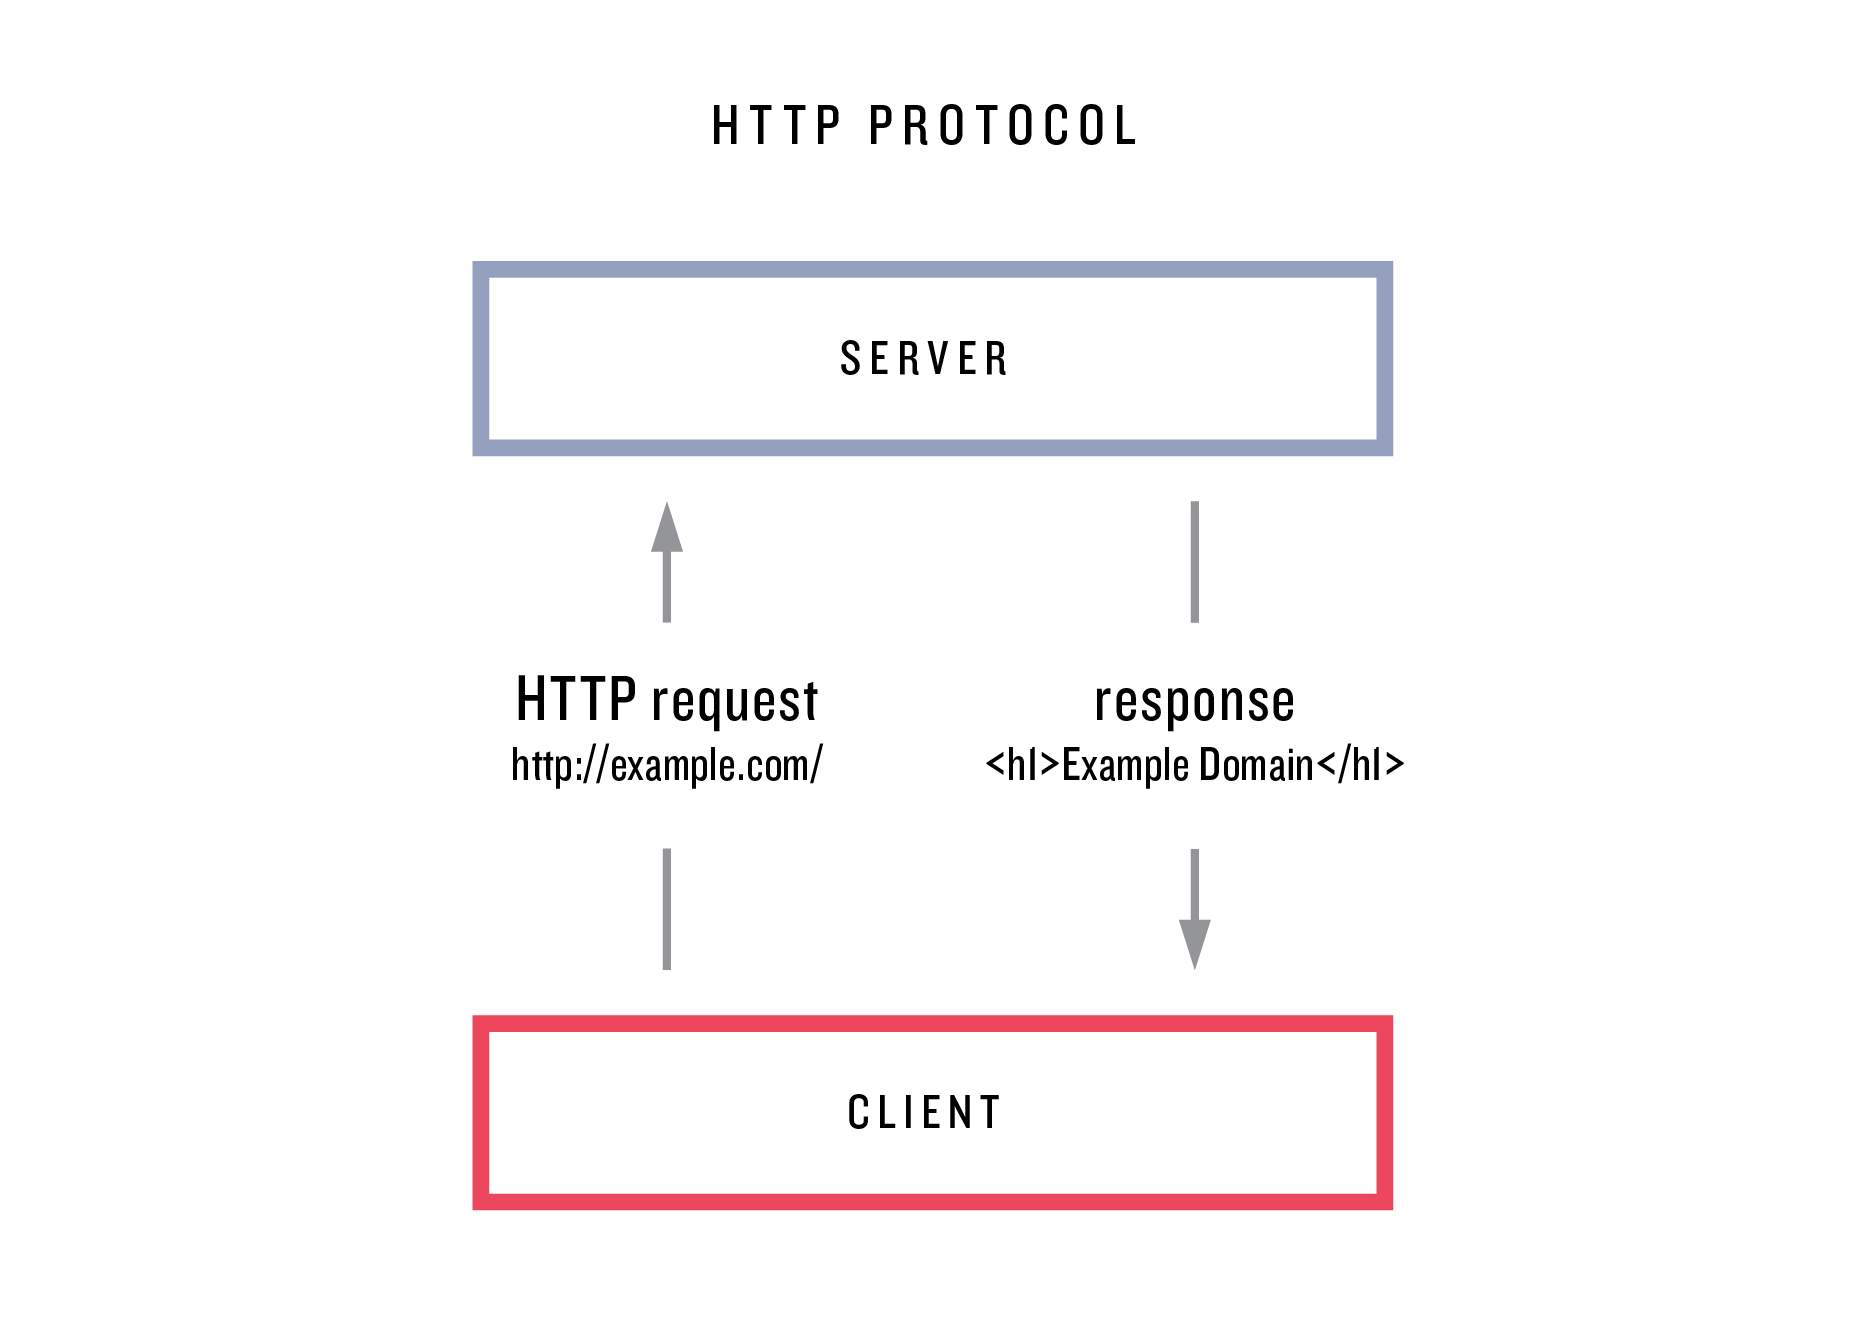
\includegraphics[height=0.4\textheight]{httpprotocol.png}
    \caption{Request-response cycle van HyperText Transfer Protocol \parencite{Hartl2019}.}
\end{figure}
Aangezien dat web applicaties niet geïnstalleerd worden is het dus wel nodig om een internetverbinding 
te hebben bij het gebruik er van. Ze worden vaak gebruikt door bedrijven om informatie en diensten 
aan hun klanten op een veilige manier aan te bieden \autocite{Nehra2023}. 
\\\\
Een web applicatie is bereikbaar door een unieke URL in te voeren in een browser 
\autocite{Beeproger2023}. Microsoft Word is een voorbeeld van een native applicatie die 
gebruikers moeten installeren op hun apparaat, in vergelijking met Google Docs dat een web applicatie 
is en dat niet geïnstalleerd moet worden \autocite{Nehra2023}.
\\\\
Web applicaties worden op dezelfde manier gemaakt als websites. Ze maken gebruik van HTML, CSS en JavaScript. 
De meeste web applicaties gebruiken een web server voor het verwerken en beheren van requests, een 
applicatieserver om de gevraagde taken te voltooien en een database om de gevraagde data 
op te halen \autocite{Varsha2023}.

\subsubsection{Voordelen van web applicaties}\label{ch:VoordelenWebApplicaties}
\paragraph{Kostprijs}
Aangezien dat één web applicatie op alle platformen draait zal dit veel goedkoper uitkomen dan bij native 
applicaties \autocite{Laarhoven2021}. Er moet namelijk maar één applicatie ontwikkeld worden die op alle 
platformen zal draaien

\paragraph{Updates}
Omdat web applicaties aan een URL gelinkt zijn, is het makkelijk om updates uit te voeren op de applicatie. 
De URL wordt vanzelf periodiek geüpdatet. Hierdoor wordt de applicatie automatisch ook up to date gehouden 
ongeacht van het platform dat een gebruiker gebruikt \autocite{Varsha2023}.

\paragraph{Installatie \& Compatibiliteit}
Daarnaast zoals gezegd, moet een web applicatie niet geïnstalleerd worden. Ze is beschikbaar op alle 
platformen en browsers. Waardoor ze zeer toegankelijk is voor gebruikers. Er is enkel een actieve 
internetverbinding nodig.

\paragraph{Integratie}
Web applicaties hebben daarnaast ook nog de mogelijkheid om makkelijk met andere web applicaties te integreren. 
Ze kunnen bijvoorbeeld met \acrshort{cms} of \acrshort{crm} systemen werken om data te beheren \autocite{Nehra2023}.

\paragraph{App store}
Er is geen goedkeuring nodig van een app store om de app te gebruiken of te updaten. Omdat een web applicatie 
via een browser wordt geopend is er zelfs geen nood voor een app store \autocite{Varsha2023}.

\paragraph{Data veiligheid}
Tot slot heeft de nood van een internetverbinding nog een voordeel. In het geval dat een apparaat
crasht of vastloopt, zullen de gegevens niet verloren gaan. Dankzij de internetverbinding worden de
gegevens automatisch opgeslagen op de server \autocite{Nehra2023}.

\subsubsection{Nadelen van web applicaties}
\paragraph{Internetverbinding}
Het grootste nadeel bij web applicaties is dat er ten alle tijde een internetverbinding nodig is om met 
de applicatie te kunnen werken \autocite{Varsha2023}. Indien er geen actieve internetverbinding aanwezig is, 
zal het niet mogelijk zijn om de applicatie te runnen.

\paragraph{Functionaliteiten}
In vergelijking met native applicaties, die gebruik kunnen maken van alle functionaliteiten van een 
apparaat is het voor web applicaties niet mogelijk om alle functionaliteiten van een apparaat te gebruiken 
\autocite{Laarhoven2021}.

\subsubsection{Verschil met een website}
Het verschil tussen een web applicatie en een website is niet altijd duidelijk. Zoals eerder gezegd 
is een web applicatie software dat toegankelijk is door er naar te surfen via een browser. 
Enkele voorbeelden van web applicaties zijn: Google apps, Amazon en Youtube. Het verschil met 
een website is dat een website een collectie is van gerelateerde web applicaties. Het bevat statische 
data zoals: foto's, tekst, audio, video's, enz... en kan bestaan uit meerdere pagina's 
\autocite{sugandha2022}. Een voorbeeld is de website van een bank waarop dat je de diensten en 
openingsuren kan zien.

\subsection{Hybride applicaties}
Het spreekt voor zich, maar een hybride applicatie is een combinatie van native en web 
applicaties \autocite{Denko2021}. Een hybride applicatie kan er identiek uitzien als een 
native applicatie echter is de manier waarop een hybride applicatie wordt gebouwd 
verschillend \autocite{Beeproger2023}. Het heeft als basis een web applicatie die in 
een soort van container wordt gestoken. Deze container zorgt er dan voor dat er in de 
applicatie een browser aanwezig is die de applicatie kan runnen. Hierdoor kan de applicatie 
ook in de app store komen waardoor het mogelijk is om hem te installeren. 
\\\\
Bedrijven maken vaak hybride applicaties als omhulsel voor een bestaande web applicatie. 
Op die manier proberen ze hun gebruikersaantal te vergroten door een aanwezigheid te hebben 
in de app store zonder al te veel moeite \autocite{Budiu2016}. 

\subsubsection{Voordelen van hybride applicaties}
\paragraph{Ontwikkelingskosten}
Omdat hybride applicaties platform onafhankelijke ontwikkeling mogelijk maakt, kunnen 
bedrijven op die manier de ontwikkelingskosten laag houden \autocite{Budiu2016}. 

\paragraph{Offline gebruik \& installatie}
Eigenlijk hebben hybride applicaties alle voordelen van web applicaties alleen krijgen ze 
nu nog eens de extra mogelijkheid om applicaties offline te gebruiken en om ze te 
installeren op een apparaat.

\subsubsection{Nadelen van hybride applicaties}
\paragraph{UI verschil}
Aangezien dat hybride applicaties op verschillende platformen kunnen werken, is het 
mogelijk dat de GUI er verschillend uitziet \autocite{sgshradha2019}. 

\paragraph{Testing}
De mogelijkheid dat hybride applicaties met zich meebrengt om te werken op alle platformen, 
zorgt ervoor dat een applicatie op al deze platformen getest moet worden \autocite{sgshradha2019}.

\paragraph{Offline gebruik}
Dankzij de combinatie van native en web applicaties, kunnen hybride applicaties ook offline 
en online werken \autocite{Khan2021}. De applicaties kunnen wel enkel offline werken als de 
applicatie niet afhankelijk is van data op een database \autocite{sgshradha2019}. Indien 
dit het geval is, kan het zijn dat de applicatie niet naar behoren werkt als er geen 
internetverbinding aanwezig is.

\subsection{Samenvatting soorten mobiele applicaties}
\begin{figure}[H]
    \centering
    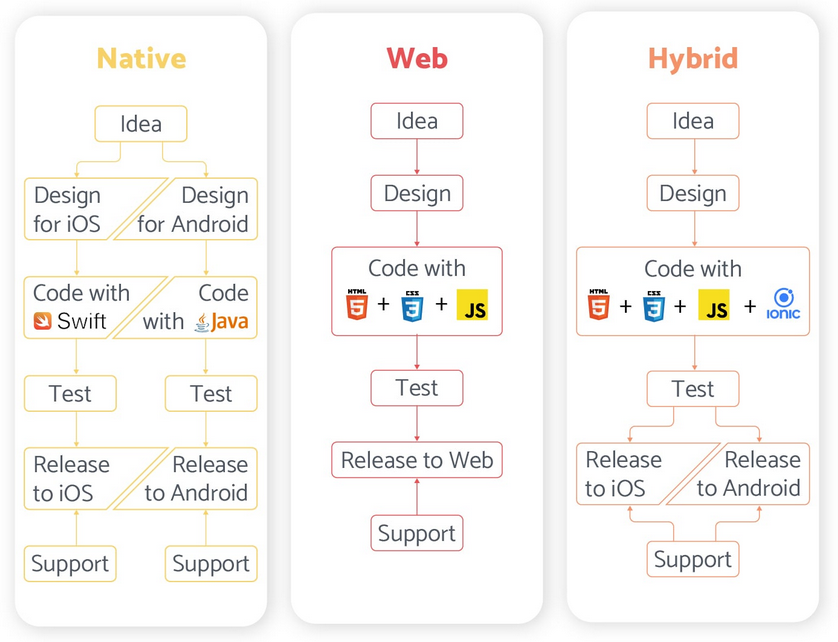
\includegraphics[height=0.4\textheight]{NativeWebHybrid2.png}
    \caption{Native vs Web vs Hybride applicaties \parencite{Merenych2021}.}
    \label{fig:NativeWebHybride}
\end{figure}
Op de figuur is een mooi overzicht te zien van hoe dat de verschillende 
soorten applicaties werken. Elke soort applicatie heeft een andere manier waarop dat ze 
op een platform geïmplementeerd worden.

\section{Native ontwikkeling}
\subsection{Wat is native ontwikkeling?}\label{subsec:wat-is-native-ontwikkeling}
Native ontwikkeling is het proces om native \ref{ch:native-applicaties} applicaties te maken 
voor een specifiek besturingssysteem, zoals Android of IOS. Hierbij wordt er gebruik gemaakt van de 
bijhorende programmeertalen en ontwikkelingsomgevingen die door de platformen worden aangeboden 
\autocite{Meirelles2019}. Ook kunnen ontwikkelaars zoals eerder gezegd gebruik maken van 
platform specifieke APIs die toegang verlenen tot de camera, gps, versnellingsmeter, kompas, 
lijst van contacten, enz...

\subsection{Voordelen van native ontwikkeling}
\paragraph{Schaalbaarheid}
Dankzij de flexibiliteit bij het ontwikkelen van native applicaties en het scheiden van 
de ontwikkeling er van, zijn native applicaties zeer schaalbaar \autocite{Koffer2023}. 
Ook hebben ontwikkelaars de mogelijkheid om elk platform individueel te schalen \autocite{Sakovich2023}. 

\subsection{Nadelen van native ontwikkeling}
\paragraph{Ontwikkelingsteams}
Nog een andere reden van de hoge kost of onderhoudsprijs bij native mobiele applicaties 
zullen de ontwikkelingsteams zijn. Bij het ontwikkeling van een applicatie voor beide 
platformen, zal er gewerkt moeten worden met ofwel één team met de kennis om voor beide 
platformen te ontwikkelen. Of er zal met twee teams gewerkt worden die elk een applicatie 
voor één platform maken \autocite{Kotlin2023}.

\paragraph{Onderhoudstijd}
Na het ontwikkelen van een native applicatie kan het zijn dat er wijzigingen komen of 
dat er updates moeten gebeuren. Aangezien dat er niet wordt gewerkt met één centraal codebase, maar 
met twee onafhankelijke projecten, zullen de wijzigingen of updates op beide projecten 
uitgevoerd moeten worden \autocite{Kotlin2023}.

\subsection{Programmeertalen en frameworks voor native ontwikkeling}
Zoals reeds hebben besproken, gaat native ontwikkeling een applicatie ontwikkelen 
specifiek voor één besturingssysteem. Om die 
applicatie kunnen verscheidene programmeertalen, frameworks 
en \acrshort{ide} gebruikt worden. Deze zijn allemaal specifiek voor ofwel Android of IOS. In de volgende 
secties gaan we enkele programmeertalen overlopen die gebruikt kunnen worden om het onderzoek uit te voeren.

\subsubsection{Android programmeertalen}
\paragraph{Java}
Java is een all-round programmeertaal met meerdere doeleinden. Eén van die doeleinden 
onder andere is Android applicatie ontwikkeling. Het was de eerste officiële programmeertaal 
voor Android applicatie ontwikkeling. Maar het blijft vandaag de dag nog steeds de 
meestgebruikte \autocite{harkiran2022}. Aangezien het de meestgebruikte programmeertaal 
is, is het soms gemakkelijker om mee te werken aangezien eventuele bugs meestal al zijn 
opgelost door de community \autocite{Thorndyke2021}. Dat wil wel niet zeggen dat het een 
gemakkelijke programmeertaal is om mee te werken. Java kan soms zeer complex zijn waardoor 
onervaren ontwikkelaars het lastig kunnen krijgen \autocite{Kesavan2021}. Daarnaast is Java 
mede door zijn complexiteit een zeer robuust programma dat een heleboel voordelen met zich 
meebrengt zoals: flexibiliteit, portabiliteit en herbruikbaarheid \autocite{Kesavan2021}.

\paragraph{Kotlin}
Momenteel is Kotlin de officiële programmeertaal voor Android applicatie ontwikkeling. 
Het is ontwikkeld door Google en \Gls{JetBrains} als lichtere en meer gebruiksvriendelijke
manier om Android applicaties te maken \autocite{Thorndyke2021}. In vergelijking met Java 
is er geen nood aan puntkomma's en is er minder code nodig om dezelfde applicatie te maken. Daarnaast laat Kotlin 
laat toe om variabelen te maken zonder ze op voorhand te moeten definiëren \autocite{Thorndyke2021}. 
Het wordt door veel bedrijven gebruikt omwille van de herbruikbaarheid van code alsook het 
gebruik van externe \gls{library} \autocite{Kesavan2021}.

\paragraph{C++}
C++ is een alternatieve methode voor Android applicatie ontwikkeling. Om C++ te gebruiken 
moet de \acrshort{andk} gebruikt worden. De applicatie kan wel niet compleet 
met C++ worden gemaakt, maar C++ en de ANDK kunnen gebruikt worden om libraries te ontwikkelen 
waarvan een applicatie gebruik maakt \autocite{harkiran2022}. Het gebruik van C++ voor libraries wordt 
vaak gedaan voor de performantie die C++ met zich meebrengt. Er moet wel rekening worden 
gehouden dat het een moeilijke programmeertaal is om te leren en dus niet voor iedereen weggelegd is 
\autocite{Designveloper2022}.

\paragraph{C\#}\label{pa:csharp}
Origineel is C\# ontwikkeld als object-georiënteerde programmeertaal, dat gebruikt zou 
worden voor desktop, mobiele en web applicaties te maken. Het was een taal die voortkwam 
vanuit C en werd ontwikkeld door Microsoft \autocite{Designveloper2022}. Het is niet alleen 
omdat het al 20 jaar bestaat, dat het daarom een populaire keuze is voor ontwikkelaars 
maar C\# heeft toegang tot het .NET framework \autocite{Kesavan2021}. Het .NET framework 
bied heel wat tools en libraries aan die helpen bij het ontwikkelen van Android applicaties. 
Daarnaast heeft C\# nog een aantal andere voordelen. C\# heeft wat cross-platform 
capaciteiten, waardoor er code overheen platformen gedeeld kan worden en er is een 
\gls{GarbageCollector}, die ervoor zorgt dat er geen geheugen lekken zijn \autocite{Patel2023}.

\paragraph{Dart}
Dart is een open-source programmeertaal, gemaakt door Google dat werd ontworpen om op 
Android platformen te runnen \autocite{Kesavan2021} met de bedoeling van klanten een 
geoptimaliseerde manier te geven om snel applicaties op het Android platform te krijgen 
\autocite{harkiran2022}. Dit wordt gedaan door te focussen op UI development. De wijzigingen 
worden snel aan de ontwikkelaar getoond dankzij de hot-reload. Tot slot is Dart ook gekend 
voor hun performantie en de mogelijkheid om te compilen tot ARM en x64 code \autocite{harkiran2022}.

\paragraph{Corona}
Ondanks dat het minder populair is, is Corona zeker geen slechte alternatief. Het is snel 
en makkelijk om te gebruiken met de capaciteiten om de meeste Android applicaties te runnen 
\autocite{Kesavan2021}. Corona is ook geen programmeertaal op zich, maar een development kit 
dat gebruikt kan worden om Android applicaties te maken door gebruik te maken van Lua. Lua is 
een lichte, efficiënte en open-source programmeertaal dat object-georiënteerd, functioneel, 
data-driven, enz. programmeren ondersteund \autocite{Lua2021}. Om met Corona te werken, worden 
er twee operationele modes gebruikt namelijk de Corona Simulator en Corona Native. De Corona 
Simulator wordt gebruikt om applicaties te maken en Corona Native wordt gebruikt om de Lua 
code te integreren met een Android Studio project om applicaties te maken die native 
functionaliteiten gebruiken \autocite{harkiran2022}.

\paragraph{Samenvatting Android programmeertalen}
Doorheen deze bachelorproef zullen we om de functionaliteiten van native Android applicaties 
te testen gebruik maken van de officiële programmeertaal van Android applicaties, 
namelijk Kotlin. Dit zullen we doen omdat Kotlin ontworpen is om veiliger te zijn dan 
sommige andere programmeertalen \autocite{Kesavan2021}, waardoor de kans op bugs en 
fouten kleiner is. Daarnaast is Kotlin makkelijk te integreren in bestaande 
Java-projecten \autocite{Kesavan2021}. Dit bespaart tijd en verhoogt de efficiëntie 
van de ontwikkeling. Tot slot heeft Kotlin een actieve gemeenschap van ontwikkelaars 
die regelmatig updates en nieuwe functies uitbrengen, waardoor de taal zich snel blijft 
ontwikkelen en verbeteren \autocite{Patel2023}.

\subsubsection{IOS programmeertalen}
\paragraph{Swift}
Swift wordt niet enkel en alleen meer gebruikt om mobiele applicaties te ontwikkelen. 
Swift wordt ook gebruikt voor besturingssystemen zoals Windows en Linux. Het werd 
ontwikkeld door Apple als een open-source opvolger van alle C gebaseerde programmeertalen 
zoals Objective-C, C++ en C \autocite{Coursera2022}. Er zijn 3 hoofdzakelijke voordelen 
waardoor Swift zeer populair is geworden bij ontwikkelaars: snelheid, veiligheid en 
introductie niveau \autocite{yuvraj2022}. Als opvolger van alle C gebaseerde programmeertalen, 
heeft het ook een betere performantie bij het uitvoeren van de meeste taken. Daarnaast kunnen 
variabelen ook aangemaakt worden zonder op voorhand een type te definiëren en puntkomma's 
zijn niet verplicht \autocite{Thorndyke2021}.

\paragraph{C\#}
Net zoals bij Android kan C\# ook gebruikt worden om IOS applicaties te ontwikkelen. 
En zoals eerder gezegd, is C\# een object-georiënteerde programmeertaal dat geïntegreerd 
is met het .NET framework \ref{pa:csharp} \autocite{yuvraj2022}. Doorheen de jaren sinds 
2000 wanneer C\# beschikbaar was heeft het heel wat populariteit gewonnen dankzij de 
eenvoudige en hoogwaardige architectuur \autocite{yuvraj2022}. Momenteel is C\# gerankt 
als de 7 populairste programmeertaal \autocite{Johns2023}. C\# gebruikt niet alleen de 
tools en libraries dat .NET te bieden heeft, maar het maakt ook gebruik van de .NET runtime 
omgeving \autocite{Pruciak2022}.

\paragraph{Objective-C}
Objective-C was de originele programmeertaal voor Apple en de fundering van MacOS en 
IOS \autocite{Johns2023}. Het is een \gls{superset} van C, het breid C dus uit en het 
voegt nieuwe functionaliteiten eraan toe \autocite{Johns2023}. Net zoals C\# is Objective-C 
een object-georiënteerde programmeertaal \autocite{Pruciak2022}. Daarnaast bestaat 
het wel al langer dan C\#, Objective-C is ontwikkeld in de vroege 1980's \autocite{Pruciak2022}. 
Aangezien het van C komt, is het ook mogelijk om C code in een Objective-C klasse toe 
te voegen. Daardoor worden Objective-C klassen simpeler, flexibeler en meer schaalbaar 
voor mobiele applicaties \autocite{yuvraj2022}. Dankzij de eenvoud en betere runtijd is 
Objective-C een van de meest gekozen programmeertalen, vooral dankzij de krachtige \acrshort{sdk} 
die worden gebruikt.

\paragraph{Samenvatting IOS programmeertalen}
Er zijn verschillende programmeertalen beschikbaar voor het ontwikkelen van IOS 
mobiele applicaties, waaronder Swift, C\# en Objective-C. Swift is de nieuwste en 
meestgebruikte programmeertaal voor IOS ontwikkeling \autocite{yuvraj2022}. Ook 
wordt Swift vaak aangeraden om mee te ontwikkelen, aangezien het mogelijk maakt om 
applicaties snel te ontwikkelen die later makkelijk uitgebreid kunnen 
worden \autocite{Pruciak2022}. 
\\\\
%TODO disclaimer
Daarom zou Swift als programmeertaal gekozen worden om te gebruiken bij het vergelijken van 
native IOS applicaties indien IOS ook in deze bachelorproef onderzocht werd.

\subsection{Tools en IDEs voor native ontwikkeling}

\paragraph{Android Studio}
Android Studio is een populaire IDE die vaak wordt gebruikt in combinatie met 
Kotlin om native Android applicaties te ontwikkelen. Het wordt vaak door ontwikkelaars 
gebruikt omwille van de ingebouwde \gls{emulator} die Android Studio bevat. Hiermee 
kunnen ontwikkelaars verschillende apparaten met verschillende Android versies uit 
testen \autocite{Medewar2022}. Daarnaast ondersteunt de emulator ook verschillende 
features die normaal enkel toegankelijk zijn bij fysieke apparaten, zoals toegang tot 
de camera, locatie, batterij instellingen, enz. \autocite{Okeke2022}. Tot slot biedt 
Android Studio ook een krachtige manier om layouts te maken. Ontwikkelaars kunnen met 
een visuele design editor schermen opbouwen in plaats van code te schrijven, die schermen 
worden dan automatisch door Android Studio omgezet naar xml bestanden \autocite{Medewar2022}. 
Het ondersteund ook GitHub integratie om makkelijk aan grote projecten te werken \autocite{Studio2023}.

\paragraph{Eclipse}
Eclipse is ontwikkeld in 2001 als een Java IDE. Maar over de jaren is het uitgegroeid 
tot een IDE dat meerdere programmeertalen ondersteund \autocite{Medewar2022}. Ondanks 
de ondersteuning van meerdere programmeertalen wordt het nog altijd vaak gebruikt om native 
Android applicaties te ontwikkelen. Het laat ook net zoals Android Studio ontwikkelaars toe 
om makkelijk te werken aan projecten dankzij de GitHub integratie \autocite{Okeke2022}, maar 
het ondersteund ook andere integratiemethoden zoals Maven \autocite{Medewar2022}. Tot slot 
bestaat er dankzij de populariteit een grootte community rondom Eclipse dat meewerkt aan de 
verbetering ervan \autocite{Medewar2022}.

\paragraph{Xcode}
Xcode is een IDE dat wordt gebruikt om software en applicaties te maken voor IOS, macOS, 
iPadOS, watchOS en tvOS \autocite{jahnavisarora2020}. Net zoals bij Android Studio en 
Eclipse bevat ook Xcode een Source Control menu waarmee ontwikkelaars makkelijk met GitHub 
kunnen werken \autocite{Medewar2022}. Om software voor alle Apple gerelateerde besturingssystemen 
te schrijven wordt er gebruik gemaakt van Swift, C, C++ en Objective C compilers 
\autocite{jahnavisarora2020}. Wat Xcode zo populair maakt is de geïntegreerde workflow 
voor coderen, testen, debuggen en ontwerpen van gebruikersinterfaces \autocite{jahnavisarora2020}.

\paragraph{Samenvatting Tools en IDEs}
Voor Android hebben we keuze tussen 2 populaire en krachtige IDEs. Maar omdat we bij Android 
gebruik maken van Kotlin als programmeertaal zullen we ook gebruik maken van Android Studio. 
Ook kiezen we voor Android Studio omdat het door Google aan ontwikkelaars wordt aangeraden 
\autocite{Medewar2022}.
\\\\
%TODO disclaimer
Bij IOS zijn er nog een heleboel IDE die ontwikkelaars kunnen gebruiken die hier niet benoemd 
worden. Desondanks zouden we indien IOS onderzocht werd in deze bachelorproef Xcode gebruiken 
in combinatie met Swift.

\section{Cross-platform ontwikkeling}

\subsection{Wat is cross-platform ontwikkeling?}
Cross-platform ontwikkeling is het proces om native applicaties \ref{ch:native-applicaties} 
te maken voor een specifiek besturingssysteem, zoals Android en IOS. Cross-platform wordt 
gebruikt om het platform specifiek probleem van native applicaties op te lossen door beide 
applicaties te ontwikkelen vanuit één codebase \autocite{Khan2021}.

\subsection{Nadelen van cross-platform ontwikkeling}
Bij cross-platform ontwikkeling is het niet mogelijk om gebruik te maken van sommige 
functionaliteiten van een apparaat \autocite{Terekhov2022}. Daarnaast kan native 
ontwikkeling indien een apparaat een nieuwe functionaliteit aanbied hier onmiddellijk gebruik 
van maken in vergelijking met cross-platform dat moet wachten op updates voor cross-platform 
ontwikkeling \autocite{Sakovich22023}.

\subsection{Voordelen van cross-platform ontwikkeling}
Net zoals bij web applicaties \ref{ch:VoordelenWebApplicaties}, zal ook bij cross-platform 
ontwikkeling de kostprijs van een applicaties lager liggen dan bij native ontwikkeling. 
Dit omdat er maar één applicatie ontwikkeld moet worden in plaats van twee. Ook zullen de 
onderhoudskosten lager liggen voor dezelfde reden \autocite{Terekhov2022}. Nog een ander 
groot voordeel van de gedeelde codebase voor twee applicaties is de gedeelde logica ervan. 
Aangezien er maar één codebase is zal de logica voor beide applicaties overeenkomen, waarbij 
dat bij native ontwikkeling soms niet het geval is \autocite{Kotlin2023}.

\subsubsection{Verschil met native ontwikkeling}
Het grootste verschil met native ontwikkeling is dat er bij cross-platform maar één 
programmeertaal en IDE nodig is om mobiele applicaties voor zowel Android als IOS te 
ontwikkelen \autocite{Hu2021}. Bij native ontwikkeling is er voor elk platform een 
programmeertaal en IDE nodig. 

\subsection{Frameworks voor cross-platform ontwikkeling}
Om cross-platform te ontwikkelen kunnen we gebruik maken van verscheidene frameworks en 
IDEs. In de volgende secties gaan we enkele overlopen waarvan we gebruik kunnen maken 
doorheen de bachelorproef om het onderzoek uit te voeren.

\paragraph{Flutter}
Flutter is een open-source framework ontwikkeld door Google dat de ontwikkeling toelaat 
van niet alleen Android en IOS applicaties, maar ook Linux, macOS, Fuchsia en Windows 
vanuit één codebase \autocite{Okeke2022a}. Het is vooral populair bij ontwikkelaars 
dankzij de simpelheid om te gebruiken en de performantie \autocite{Sakovich22023}. De 
hoge performantie komt door het gebruik van C en C++ \autocite{Terekhov2022}. Daarnaast 
heeft het ook een \gls{Hotreload} waardoor ontwikkelaars snel resultaten kunnen zien bij 
veranderingen in de code \autocite{Sakovich22023}.

\paragraph{React native}
React native is net zoals Flutter een open-source framework ontwikkeld door Facebook. 
Het laat toe om IOS en Android applicaties te ontwikkelen \autocite{Terekhov2022}. 
Het grootste voordeel van React native is de ontwikkeltijd waarmee applicaties ontwikkeld 
kunnen worden \autocite{Terekhov2022}, de grote community die meehelpt aan het ontwikkelen 
van externe libraries \autocite{Okeke2022a}. Dankzij die externe libraries hebben ontwikkelaars 
toegang tot native features die normaal voor cross-platform ontwikkeling niet toegankelijk is. 
Deze externe libraries kunnen geschreven zijn in Objective-C, Swift of Java \autocite{Okeke2022a}. 
Tot slot heeft React native ook een hot reload functie net zoals flutter waardoor ontwikkelaars 
snel resultaten kunnen zien bij veranderingen in de code \autocite{Terekhov2022}.

\paragraph{.NET MAUI (vroeger Xamarin)}
.NET MAUI is net zoals Flutter en React native een open-source framework ontwikkeld door 
Microsoft. Het maakt gebruik van C\# als programmeertaal en het .NET framework voor 
native libraries \autocite{Sakovich22023}. Net zoals bij Flutter en React native bezit 
ook .NET MAUI over een hot reload functie om snel te kunnen ontwikkelen en debuggen. 
Dankzij het gebruik van C\# bezit ook .NET MAUI net zoals Flutter en React native over 
een hoge performantie \autocite{Okeke2022a}. Wel een groot nadeel is dat applicaties 
niet altijd compatibel zijn met de laatste versies van Android of IOS \autocite{Terekhov2022}.

\paragraph{Samenvatting frameworks}
Ze staan hier niet allemaal beschreven maar er zijn nog een heel wat frameworks die 
gebruikt kunnen worden voor cross-platform ontwikkeling. Maar de drie frameworks die 
hier beschreven zijn hebben allemaal een gelijkaardige performantie. React native en 
.NET MAUI hebben ook makkelijk toegang tot native features dankzij de native libraries. 
Uit deze drie frameworks gaan we React native kiezen om cross-platform te ontwikkelen 
dankzij de performantie, native libraries en grote community er rond. React native 
bevat voor deze bachelorproef de beste eigenschappen om het onderzoek uit te voeren.

\subsection{IDEs voor cross-platform ontwikkeling}

\paragraph{Visual Studio Code}
Er is maar één IDE die eruit springt en dat is Visual Studio Code. Het is een 
universele IDE die gebruikt kan worden voor alle programmeertalen. Daarnaast is er een 
groot aanbod van extensies die het mogelijk maken om de IDE aan te passen aan de 
specifieke behoefte van de ontwikkelaar \autocite{Heller2022}. Daarom zullen we Visual 
Studio Code gebruiken als IDE om cross-platform te ontwikkelen.

\section{Functionaliteiten}
\subsection{Keuze te onderzoeken functionaliteiten}
Om een vergelijking te kunnen maken tussen native en cross-platform ontwikkeling, 
hebben we een aantal functionaliteiten nodig om te onderzoeken. 

\paragraph{Basisfunctionaliteiten}
Dit omvat functionaliteiten die elke mobiele applicatie zou moeten hebben. Zoals 
het openen van de app met ondertussen een laadscherm tonen. Daarnaast het navigeren 
tussen verschillende schermen binnen de applicatie. Deze functionaliteiten zijn bij 
elke applicatie aanwezig en vormen dus een belangrijk onderdeel van de gebruikerservaring 
en daarom ook een belangrijk onderdeel van de vergelijking tussen native en cross-platform.
Hierbij zullen we vooral kijken naar het invloed op de opstartsnelheid van de applicatie 
en de snelheid waarmee er genavigeerd kan worden tussen de verschillende schermen.

\paragraph{Audio- en videospelers}
Een mobiele app kan verschillende soorten media afspelen, zoals video's en muziek. 
Hierbij zullen we kijken naar de implementatie van deze functionaliteit in 
zowel native als cross-platform ontwikkeling. We zullen de integratie van externe bibliotheken 
voor het afspelen van media en video's en hun performantie onderzoeken.

\paragraph{Gebruik van sensoren}
Mobiele apparaten bevatten verschillende sensoren, zoals de accelerometer en gyroscoop. 
Ze kunnen worden gebruikt in mobiele applicaties om bijvoorbeeld beweging te detecteren 
of de oriëntatie van het apparaat. Bij het gebruik van sensoren kijken we naar hoe deze 
sensoren geïmplementeerd kunnen worden en de snelheid waarmee data ingelezen kan worden 
in zowel native als cross-platform ontwikkeling.

\paragraph{Notificaties}
Notificaties (meldingen) zijn berichten die worden weergegeven op het scherm van een 
apparaat. Ze kunnen komen via het internet of door een applicatie zelf. We zullen hierbij 
kijken naar de implementatie van enkel lokale notificaties. Aangezien de performantie van 
push-notificaties gedeeltelijk zal afhangen van een extern framework of netwerk waarover 
dezelfde performantie niet gegarandeerd kan worden.

% %\paragraph{Locatie}
% %\paragraph{func7}
% %\paragraph{func8}
% %\paragraph{func9}
% %\paragraph{func10}

\section{Samenvatting stand van zaken}
Nu dat er een inzicht verkregen is in mobiele applicaties en de ontwikkeling ervan, 
kunnen we van start gaan met het onderzoek. We zullen alle opgelijste functionaliteiten 
voor zowel native als cross-platform ontwikkelen. Bij native ontwikkeling zullen we 
Kotlin en Android Studio gebruiken om native applicaties voor Android te maken. 
Bij cross-platform zullen we React-native en Visual Studio Code gebruiken om de 
native applicaties te maken.















%%=============================================================================
%% Methodologie
%%=============================================================================

\chapter{Methodologie}
\label{ch:methodologie}

%% TODO: Hoe ben je te werk gegaan? Verdeel je onderzoek in grote fasen, en
%% licht in elke fase toe welke stappen je gevolgd hebt. Verantwoord waarom je
%% op deze manier te werk gegaan bent. Je moet kunnen aantonen dat je de best
%% mogelijke manier toegepast hebt om een antwoord te vinden op de
%% onderzoeksvraag.

Zoals elk onderzoek start ook dit onderzoek met een uitgebreide literatuurstudie van wat mobiele applicaties zijn, 
hoe dat ze worden ontwikkeld en welke functionaliteiten onderzocht gaan worden. Deze literatuurstudie is te vinden in Hoofdstuk \ref{ch:stand-van-zaken}.
\\\\
Vervolgens wordt er in hoofdstuk \ref{ch:ontwikkelomgeving} gekeken hoe dat we de ontwikkelomgeving opstellen om met Kotlin in Android Studio 
te werken en met React native in Visual Studio Code.
\\\\
Na het opstellen van de ontwikkelomgeving wordt er in hoofdstuk \ref{ch:projecten} uitgelegd hoe dat we de blanco projecten aanmaken. 
Deze blanco projecten worden dan doorheen de bachelorproef gebruikt om functionaliteiten uit te werken.
\\\\
Daarna zullen alle functionaliteiten uitgewerkt worden tot een project, hier wordt dan ook de ontwikkeltijd van een functionaliteit 
gedocumenteerd met daarbij eventuele bugs of problemen. Ook wordt hier de performantie van de functionaliteiten gemeten. 
En de eventuele mogelijkheid om op te schalen zal hier ook bekeken worden. Elke functionaliteit wordt opgedeeld in zijn eigen hoofdstuk. 
Op die manier kunnen de resultaten per functionaliteit duidelijk teruggevonden worden.
\begin{itemize}
    \item Hoofdstuk \ref{ch:basisfunctionaliteiten} voor de basisfunctionaliteiten
    \item Hoofdstuk \ref{ch:camera} voor de camera-integratie
    \item Hoofdstuk \ref{ch:sensoren} voor het gebruik van sensoren
    \item Hoofdstuk \ref{ch:notificaties} voor de push-notificaties
    \item Hoofdstuk \ref{ch:audioenvideo} voor de audio- en videospelers
\end{itemize}
Tot slot worden de resultaten en individuele conclusies van alle functionaliteiten uit de vorige hoofdstukken opgelijst en samengevat 
in hoofdstuk \ref{ch:conclusie} om een antwoord te geven op de onderzoeksvragen uit hoofdstuk \ref{ch:inleiding}.

\section{Volgorde onderzoek}
Voor de functionaliteiten te onderzoeken zullen we hetzelfde stappenplan volgen per functionaliteit. 
\begin{enumerate}
    \item Blanco project aanmaken.
    \item Ontwikkeltijd meten.
    \begin{enumerate}
        \item Duurtijd van functionaliteit implementeren.
        \item Duurtijd van eventuele bugs of problemen.
    \end{enumerate}
    \item Performantie van functionaliteit meten.
    \item Mogelijkheid om op te schalen onderzoeken.
    \item resultaten formuleren.
\end{enumerate}
We zullen beginnen door een blanco project aan te maken. Daarna zullen we op dit blanco project de functionaliteit in kwestie implementeren. 
Hierbij gaan we dan de tijd nodig om de functionaliteit te implementeren meten en ook eventuele bugs of problemen. 
Na het implementeren van de functionaliteit zullen we bij beide applicaties de performantie meten. 
Daarna gaan we kijken of dat de functionaliteit opgeschaald kan worden, hoe moeilijk of makkelijk dit kan gebeuren en hoe dat dit moet gebeuren. 
Tot slot zullen we dan per functionaliteit een conclusie formuleren op basis van de verkregen resultaten.

\section{Hoe word er getest}
\subsection{Performantie}
\paragraph{Android Studio}
Om de performantie van de native applicaties te meten maken we gebruik van Android Studio. 
Android Studio bied de tool Android profiler aan die het mogelijk maken om de performantie in kaart te brengen. 
Deze tool kunnen we openen met \textit{View > Tool Windows > Profiler}. %TODO foto invoegen
Deze tool stelt ons in staat om de performantie van applicaties tijdens het uitvoeren op een emulator te analyseren en meten. 
Het geeft ons gedetailleerde inzichten in verschillende prestatieaspecten, zoals CPU-gebruik, geheugengebruik, netwerkactiviteit en energieverbruik. 
Met de Android Profiler kunnen we ook realtime grafieken genereren en de gegevens bekijken. 
\\\\
Doorheen dit onderzoek zullen we gebruik maken van de CPU-profiler en geheugenprofiler om de performantie te meten.

\subparagraph{CPU-profiler}
Hiermee kunnen we de CPU-activiteiten van de applicaties meten. Op die manier kunnen we zien welke threads en methoden de CPU gebruiken en ook hoelang dat ze deze gebruiken.

\subparagraph{Geheugenprofiler}
Hiermee kunnen we het geheugengebruik van de applicaties meten. We kunnen de geheugenallocatie en deallocatie volgen en de geheugenprofielen analyseren. 
Op deze manier kunnen we de impact van de applicatie op het geheugengebruik begrijpen.

\paragraph{React native}
Om de performantie van de cross-platform applicaties te meten maken we gebruik van de Performance Monitor tool. 
Deze is beschikbaar via de React native Developer Tools. Naast de Performance Monitor bieden de React native Developer Tools ook nog andere tools aan zoals: 
Element Inspector, Network Inspector, Console Logging en Redux Debugger. Binnen dit onderzoek gaan we enkel gebruik maken van de Performance Monitor. 
Deze zullen we net zoals bij Android Studio gebruiken om het CPU- en geheugengebruik van cross-platform applicaties te meten en analyseren.

\subsection{Schaalbaarheid}
TODO

\subsection{Ontwikkeltijd}
TODO


% Voeg hier je eigen hoofdstukken toe die de ``corpus'' van je bachelorproef
% vormen. De structuur en titels hangen af van je eigen onderzoek. Je kan bv.
% elke fase in je onderzoek in een apart hoofdstuk bespreken.

%%=============================================================================
%% Opstellen ontwikkelomgeving
%%=============================================================================

\chapter{Opstellen ontwikkelomgeving}%
\label{ch:ontwikkelomgeving}

Vooraleer het onderzoek van start kan gaan, moet de ontwikkelomgeving voor zowel native 
als cross-platform opgesteld worden. 
\\\\
Zoals besproken in hoofdstuk \ref{ch:stand-van-zaken} zal voor native ontwikkeling Kotlin 
met Android Studio gebruikt worden om applicaties te ontwikkelen. Voor cross-platform zal React Native 
met Visual Studio Code gebruikt worden.

\section{Opstellen native ontwikkeling}\label{se:native}

Om met native ontwikkeling van start te gaan zullen we eerst Android Studio moeten downloaden. 
Dit kan vanop de website \url{https://developer.android.com/studio/}

\paragraph{1. Components}
Bij het eerste scherm van het installatieprogramma is het belangrijk om ook 
\textbf{Android Virtual Device} te selecteren. Deze stelt ons in staat om de applicaties die we 
zowel voor native als cross-platform zullen ontwikkelen kunnen runnen. 

\paragraph{2. Installatie locatie}
Op het volgend scherm kiezen we de locatie waar Android Studio geïnstalleerd wordt. 
Het is aangeraden om dit niet te vervangen omdat React native gebruik maakt van de standaard 
locatie om bepaalde componenten op te zoeken. 

\paragraph{3. Startmenu map}
Deze is zelf te kiezen. Hiermee creëer je een shortcut vanwaar Android Studio kan worden opgestart.

\paragraph{4. Android SDK}\label{par:sdk}
Als de installatie goed is verlopen krijgen we volgend welkom scherm te zien. 
\begin{figure}[H]
    \centering
    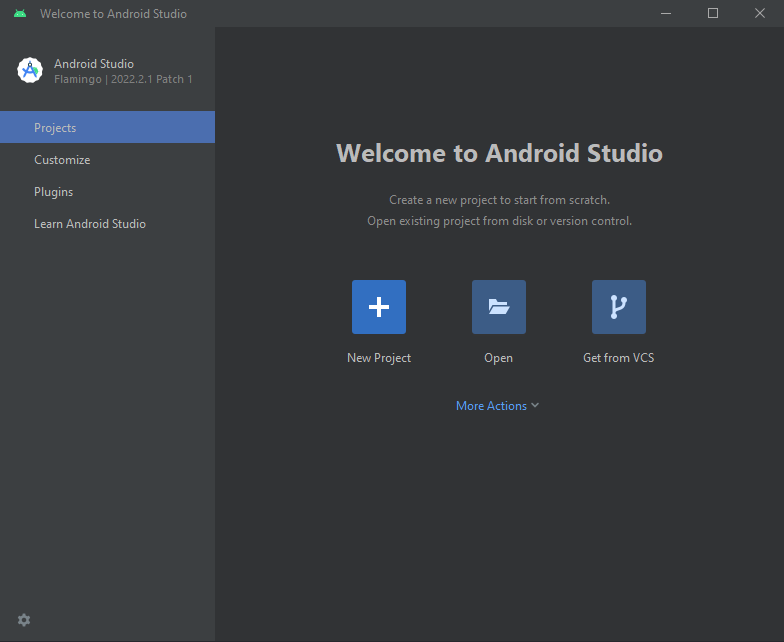
\includegraphics[height=0.4\textheight]{androidinstallatie.png}
    \caption{Startscherm na Android Studio installatie.}
\end{figure}
Standaard wordt de laatste Android SDK geïnstalleerd door Android Studio. 
Deze zullen we ook tijdens de duratie van het onderzoek gebruiken. 
Maar om met deze laatste Android SDK te werken hebben we Android 13 (Tiramisu) nodig. 
Om deze te installeren drukken we op \textit{More Actions}. Op het nieuwe verkregen scherm 
kunnen we dan Android 13 (Tiramisu) aanvinken. Ook zullen we onderaan rechts het vakje 
\textbf{Show Package Details} aanvinken om dan te verifiëren dat ook zeker 
\textbf{Android SDK Platform 33}, \textbf{Sources for Android 33} en 
\textbf{Google APIs Intel x86\_64 Atom System Image} zijn aangevinkt.
\\\\
Daarna navigeren we naar SDK Tools en vinken we opnieuw \textbf{Show Package Details} 
aan en vinken we ook onder Android SDK Build-Tools \textbf{33.0.0} aan. 
Tot slot drukken we op \textbf{Apply} om de Android SDK en gerelateerde tools te downloaden en installeren. 
Maak daarna ook een dummy project aan (Empty Activity) om Android Studio van start te krijgen.

\paragraph{5. Emulator}
Om de applicaties die we zullen ontwikkelen te runnen hebben we een emulator nodig. 
Deze kunnen we aanmaken bovenaan rechts \textit{Device Manager > Create device}. 
Eerst en vooral selecteren we de device dat we willen emuleren. Voor het onderzoek 
gaan we gebruik maken van een Pixel 3 als device. Na het selecteren van ons device moeten we 
de Android versie klikken. Hier selecteren we Tiramisu met API Level 33 (Die we daarnet hebben geïnstalleerd). 
Tot slot zijn er nog een aantal configuratie instellingen voor het apparaat. Wij laten deze allemaal op hun standaard 
waarden staan.
\\\\
Nu is Android Studio klaar om native applicaties te ontwikkelen en runnen. 


\section{Opstellen cross-platform ontwikkeling}

Om cross-platform te ontwikkelen door gebruik te maken van React native is er wat meer werk om 
de omgeving op te stellen. Eerst zullen we Visual Studio Code downloaden. 
Dit kan vanop de website \url{https://code.visualstudio.com/download} 

Na het installeren van Visual Studio Code kunnen we de React native ontwikkelomgeving opstellen. 
Dit kan door de handleiding te volgen vanop de website \url{https://reactnative.dev/docs/environment-setup}.

\paragraph{1. React Native CLI Quickstart}
Voor de React native ontwikkelomgeving kunnen we ook gebruik maken van Expo. 
Dit is een simpele manier om snel applicaties visueel werkend te krijgen. 
Maar voor dit onderzoek zullen we de applicaties op dezelfde emulator runnen waarop de native 
ontwikkelde applicaties runnen. Hiervoor volgen we de React Native CLI Quickstart handleiding. 

\paragraph{2. Besturingssysteem en doelsysteem}
Afhankelijk van het gebruikte besturingssysteem is er een andere handleiding. 
Doorheen dit onderzoek zullen we werken op een Windows laptop en zullen we focussen op Android applicaties.

\paragraph{3. Node \& JDK}
Als eerste moeten we \Gls{Node} en \acrshort{jdk} installeren. Dit kunnen we makkelijk 
doen met \Gls{Chocolatey}. Chocolatey indien niet geïnstalleerd kan worden gedownload 
vanop de website \url{https://chocolatey.org/install}. Eerst openen we een 
opdrachtprompt (powershell) als administrator waaraan we volgende commando meegeven.
\begin{minted}{bash}
choco install -y nodejs-lts microsoft-openjdk11
\end{minted}
Voor Node gebruiken we de laatste versie. De minimale versie waarmee React native kan werken is 14. 
Voor de JDK gebruiken we versie 11 aangezien hogere versies voor problemen kunnen zorgen.

\paragraph{4. Android ontwikkelomgeving}
Net zoals bij native ontwikkeling hebben we voor React native applicaties ook Android Studio nodig. 
Dit is omdat we om de applicatie te runnen gebruik maken van de emulator binnenin Android Studio. 
Android Studio zelf wordt niet direct gebruikt maar er wordt enkel gebruik gemaakt van de 
emulator die Android Studio aanbied.
\\\\
Bij het opstellen van de React native omgeving zijn er een paar instellingen waar we rekening 
mee moeten houden. Maar hiermee is al rekening gehouden bij het installeren van Android Studio 
in paragraaf \ref{par:sdk}.

\paragraph{5. ANDROID\_HOME omgevingsvariabelen}
De React native tools hebben enkele omgevingsvariabelen nodig om native applicaties te bouwen. 
Om deze omgevingsvariabelen in te stellen openen we eerst het configuratiescherm van Windows. 
Daarna gaan we naar 
\textit{Gebruikersaccounts > Gebruikersaccounts > Mijn omgevingsvariabelen veranderen > Nieuw\dots}. 
In het nieuwe verkregen scherm vullen we dan de naam van de omgevingsvariabel \textbf{ANDROID\_HOME} 
en de path naar de Android SDK in. De standaard path naar de Android SDK is 
\textbf{\%LOCALAPPDATA\%\backslash Android\backslash Sdk}. 
De locatie van de Android SDK is ook te vinden via Android Studio via 
\textit{File > Settings > Appearance \& Behavior > System Settings > Android SDK}.
\\\\
Om te controleren dat de omgevingsvariabel correct is toegevoegd openen we een nieuwe 
opdrachtprompt (powershell) en geven we volgend commando in.
\begin{minted}{bash}
Get-ChildItem -Path Env:\
\end{minted}
In de teruggegeven lijst controleren we dan of dat ANDROID\_HOME effectief is toegevoegd.
\\\\
Tot slot moeten we de \textbf{Path} omgevingsvariabel aanpassen. 
Opnieuw navigeren we in het configuratiescherm naar het overzicht met alle omgevingsvariabelen 
\textit{Gebruikersaccounts > Gebruikersaccounts > Mijn omgevingsvariabelen veranderen}. 
Hierin selecteren we de Path omgevingsvariabel en daarna drukken we op \textit{Bewerken...}. 
Bij het nieuw verkregen scherm drukken we op \textit{Nieuw} en voegen we de path naar platform-tools 
toe aan de lijst. Het path van de platform-tool is standaard 
\textbf{\%LOCALAPPDATA\%\backslash Android\backslash Sdk\backslash platform-tools}.

\paragraph{6. React native Command Lin Interface (CLI)}
React native heeft een ingebouwde command line interface (CLI) om te werken met React native. 
Deze kan gebruikt worden dankzij Node.js dat we daarnet installeerden.
\begin{minted}{bash}
npx react native [commando]
\end{minted}

\paragraph{7. Emulator gebruiken} \label{par:emulatorgebruiken}
Om nu effectief applicaties te laten runnen maken we gebruik van de emulator die Android Studio aanbied. 
Aangezien deze al opgesteld is bij het opzetten van Android Studio \ref{se:native} 
moeten we dit niet meer doen voor React native. Om de applicatie starten hebben we twee terminals nodig 
binnen Visual Studio code, deze kunnen we openen via \textit{Terminal > New Terminal}. 
In de eerste terminal starten we \Gls{Metro} met het volgende commando.
\begin{minted}{bash}
npx react-native start
\end{minted}
In de tweede terminal geven we het volgende commando dat de applicatie zal opbouwen en 
deployen naar de emulator.
\begin{minted}{bash}
npx react-native run-android
\end{minted}

\section{Gebruikte hardware tijdens onderzoek}

Doorheen het onderzoek zullen alle projecten starten vanuit een blanco project en op dezelfde emulator 
getest worden. Deze emulator zal altijd runnen op hetzelfde apparaat. Dankzij volgend commando 
kunnen we de informatie verkrijgen van een apparaat:
\begin{minted}{bash}
npx react-native info
\end{minted}
Deze geeft bij het gebruikte apparaat voor dit onderzoek volgende output:
\begin{minted}{bash}
System:
    OS: Windows 10 10.0.19044
    CPU: (12) x64 AMD Ryzen 5 5600H with Radeon Graphics
    Memory: 2.90 GB / 15.86 GB
Binaries:
    Node: 18.16.0 - C:\Program Files\nodejs\node.EXE
    Yarn: Not Found
    npm: 9.5.1 - C:\Program Files\nodejs\npm.CMD
    Watchman: Not Found
SDKs:
    Android SDK: Not Found
    Windows SDK: Not Found
IDEs:
    Android Studio: AI-222.4459.24.2221.9971841
    Visual Studio: Not Found
Languages:
    Java: 11.0.18
npmPackages:
    @react-native-community/cli: Not Found
    react: 18.2.0 => 18.2.0 
    react-native: 0.71.7 => 0.71.7 
    react-native-windows: Not Found
    npmGlobalPackages:
    *react-native*: Not Found
\end{minted}
Voor dit onderzoek wordt een apparaat met een AMD Ryzen 5 5600H processor 
met 12 cores, geïntegreerde Radeon Graphics en 16GB RAM geheugen gebruikt, wat sterk en snel 
genoeg is om het onderzoek uit te voeren.











%%=============================================================================
%% Opstellen projecten
%%=============================================================================

\chapter{Aanmaken blanco project}%
\label{ch:projecten}

Na het opzetten van de ontwikkelomgeving voor zowel native als cross-platform wordt 
in dit hoofdstuk uitgelegd hoe een blanco project wordt aangemaakt.

\section{Android Studio}

Android Studio kan als IDE zelf nieuwe projecten aanmaken met \textit{File > New > New Project\dots}. 
Hierna wordt een overzicht getoond van projecten die als basis kunnen worden gebruikt. Ook 
kan er op dit scherm gekozen worden voor welk apparaat de applicatie is.
\begin{figure}[H]
    \centering
    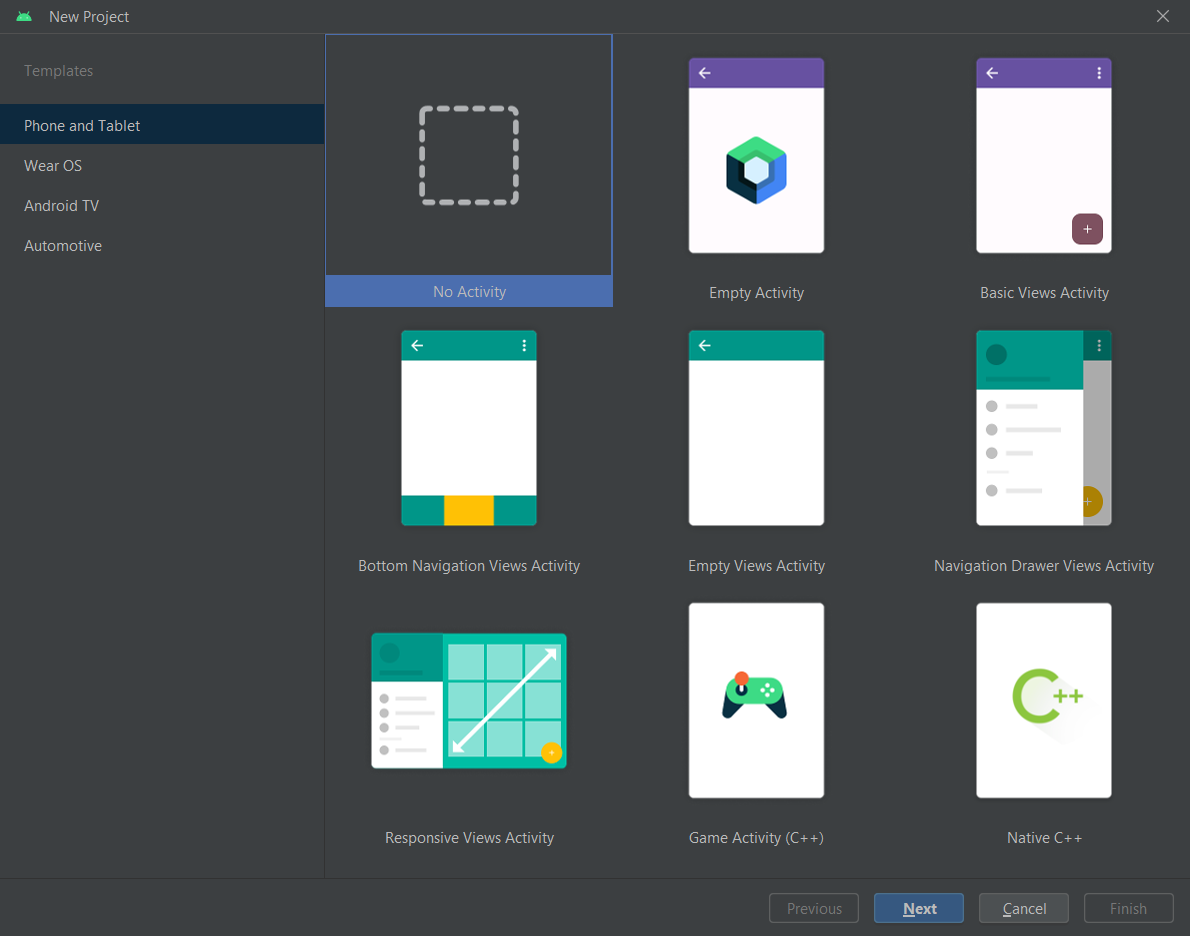
\includegraphics[height=0.35\textheight]{OverzichtProjecten.png}
    \caption{Overzicht startprojecten Android Studio.}
\end{figure}
Afhankelijk van de functionaliteit die wordt geïmplementeerd, zal een ander 
startproject gekozen worden. Na het kiezen van het startproject kan een naam, 
programmeertaal en de minimaal ondersteunde Android API worden ingegeven. Voor dit onderzoek wordt er gekozen 
voor Kotlin. De naam en minimale ondersteunde Android API spelen hierbij geen rol.

\subsection{Basisfunctionaliteiten}
\label{par:basisfunctionaliteiten}
Bij de basisfunctionaliteiten wordt
\textbf{Bottom Navigation Views Activity} als startproject gebruikt om te kunnen navigeren tussen 
verschillende schermen. Daardoor moeten er geen extra libraries worden geïmplementeerd.

\subsection{Overige functionaliteiten}
Voor de overige functionaliteiten (gebruik van sensoren, 
push-notificaties en audio- en videospelers) wordt
\textbf{Empty Views Activity} als startproject gebruikt. Op die manier zal er zo weinig mogelijk 
\gls{overhead} zijn die de resultaten kan beïnvloeden.

\subsection{Firebase Performance Monitoring}
Om de performantie van de applicaties te meten, meer specifiek de tijdsduur 
die een stuk code nodig heeft om uit te voeren, 
wordt de Firebase Performance Monitoring tool in het project geïmplementeerd. 

\paragraph{Firebase aan project toevoegen}
Vooraleer de Performance Monitoring tool geïmplementeerd kan worden, moet Firebase 
aan het project worden toegevoegd.

\subparagraph{1. Configuratie bestanden toevoegen}
In het Firebase project voegen we een nieuwe Android applicatie toe. Om deze aan te maken geven we de package naam 
dat te vinden is in build.gradle(module) bestand als applicationId en optioneel de naam van de applicatie mee.
\\\\
Na dat de Android applicatie is aangemaakt, moeten we het \textbf{google-services.json} bestand downloaden. 
Deze plaatsen we dan in de \textit{app} folder.

\subparagraph{2. Firebase plugins configureren}
Om Firebase het configuratiebestand nu te laten gebruiken moeten we de google-services plugin toevoegen aan 
de dependancies in het build.gradle(project) bestand boven de plugins. 
\begin{minted}{java}
buildscript {
    repositories {
        google()
        mavenCentral()
    }

    dependencies {
        // andere dependancies
        classpath "com.google.gms:google-services:4.3.15"
    }
}
\end{minted}
Daarna moeten we de plugin uitvoeren door deze aan het build.gradle(module) bestand toe te voegen.
\begin{minted}{java}
plugins {
    // andere plugins 
    id "com.google.gms.google-services"
}
\end{minted}
Tot slot moeten we de Firebase SDKs toevoegen aan het build.gradle(module) bestand.
\begin{minted}{java}
dependencies {
    // andere dependancies
    implementation platform("com.google.firebase:firebase-bom:32.0.0")
}
\end{minted}
Firebase is nu volledig aan ons project toegevoegd.

\paragraph{Implementatie Performance Monitoring tool}
Nu Firebase aan ons project is toegevoegd, kan de Performance Monitor 
worden toegevoegd.

\subparagraph{1. Performance Monitoring SDK aan applicatie toevoegen}
Als eerst voegen we de Performance Monitor SDK toe aan ons project in het \textbf{build.gradle(module)} bestand.
\begin{minted}{java}
dependencies {
    // ... andere dependancies
    implementation "com.google.firebase:firebase-perf-ktx"
}
\end{minted}

\subparagraph{2. Performance Monitoring Gradle plugin toevoegen}
Na het toevoegen van de SDK moeten we de Perormance Monitoring Gradle plugin toevoegen. 
Dit doen we door de dependancies hiervan toe te voegen aan het \textbf{build.gradle(project)} bestand.
\begin{minted}{java}
dependencies {
    // ... andere dependancies
    classpath "com.google.firebase:perf-plugin:1.4.2"
}
\end{minted}
Tot slot voegen we de plugin toe. Dit doen we door deze in het \textbf{build.gradle(module)} bestand toe te voegen.
\begin{minted}{java}
plugins {
    // ... andere plugins
    id "com.google.firebase.firebase-perf"
}
\end{minted}
Nu is het blanco project klaar om vanuit dit project alle functionaliteiten te 
implementeren en onderzoeken, buiten de basisfunctionaliteiten. Hiervoor zullen we vanuit een ander project starten, 
maar zullen we de Perormance Monitoring tool op dezelfde manier implementeren.

\subparagraph{3. Performance meten}
Nu kunnen we een trace maken om de performantie te meten. Doorheen de applicaties zal dit er als 
volgt uitzien.
\begin{minted}{java}
val trace = FirebasePerformance.getInstance().newTrace("naam_trace")

trace.start()
// uit te voeren code
trace.stop()
\end{minted}
De trace wordt gestart voor de code die we willen meten en gestopt na de code die we willen meten.
De trace wordt dan automatisch naar de Firebase console gestuurd. Hier kunnen we de trace terugvinden
en de performantie analyseren.


\section{Cross-platform project}\label{sec:projectencross}

Om bij React Native een project op te starten, wordt volgend commando gebruikt: 
\begin{minted}{bash}
npx react-native init <projectnaam>
// Of
npx react-native@X.XX.X init <projectnaam> --version X.XX.X
\end{minted}
Deze wordt uitgevoerd in de terminal van Visual Studio Code in de gewenste map waar 
het project moet worden aangemaakt.
\\\\
Het eerste commando zal een blanco React Native project aanmaken met de laatste versie. Bij het tweede commando
kan er een versie worden meegegeven door \textbf{X.XX.X} in bovenstaande commando te vervangen.
In dit onderzoek wordt er gebruik gemaakt van de laatste beschikbare versie namelijk \textbf{0.71.7}.

\subsection{Firebase Performance Monitoring}
Om de performantie van de applicaties te meten moeten de 
Firebase Performance Monitoring tool in het project worden geïmplementeerd.

\paragraph{Firebase project aanmaken}
Vooraleer de Performance Monitoring tool geïmplementeerd kan worden moet Firebase 
aan het project worden toegevoegd.

\subparagraph{1. Dependancy installeren}
Eerst moet de React Native Firebase "app" module aan de root van het React Native project worden toegevoegd. 
Dit wordt gedaan met volgend commando:
\begin{minted}{bash}
npm install --save @react-native-firebase/app
\end{minted}

\subparagraph{2. Configuratie bestanden toevoegen}
Nadat de dependancy is toegevoegd, moet er een nieuw Firebase project worden aangemaakt. 
Om deze aan te maken moet de package naam worden meegegeven die te vinden is in het 
\textit{android/app/build.gradle} bestand als 
\textbf{applicationId}. Optioneel kan de naam van de applicatie mee worden gegeven.
\\\\
Nadat de Android applicatie is aangemaakt, moet het \textbf{google-services.json} bestand worden gedownload. 
Deze wordt dan geplaatst in de \textit{android/app} folder.

\subparagraph{3. Firebase configureren}
Om Firebase het configuratiebestand nu te laten gebruiken, moet de google-services plugin worden toegevoegd aan 
de dependancies binnen het \textit{android/build.gradle} bestand. 
\begin{minted}{java}
buildscript {
    dependencies {
        // andere dependencies
        classpath "com.google.gms:google-services:4.3.15"
    }
}
\end{minted}
Tot slot moet de plugin aan het \textit{android/app/build.gradle} bestand worden toegevoegd.
\begin{minted}{java}
apply plugin: "com.google.gms.google-services"
\end{minted}
En worden deze ook aan de dependancies toegevoegd in hetzelfde \textit{android/app/build.gradle} bestand.
\begin{minted}{java}
dependencies {
    // andere dependancies
    implementation platform("com.google.firebase:firebase-bom:32.0.0")
}
\end{minted}
De React Native Firebase app module is nu volledig geïmplementeerd.

\paragraph{Implementatie Performance Monitoring tool}
Nu de React Native Firebase app module is geïmplementeerd, zijn alle voorwaarden voldaan om de 
Performance Monitoring tool verder te implementeren.

\subparagraph{1. Dependancy installeren}
Eerst moet de Performance Monitoring tool aan de root van ons project worden toegevoegd. 
Dit wordt gedaan met volgend commando:
\begin{minted}{bash}
npm install --save @react-native-firebase/perf
\end{minted}

\subparagraph{2. Performance Monitoring tool configureren}
Daarnaast moet de plugin worden toegevoegd aan 
de dependancies binnen het \textit{/android/build.gradle} bestand. 
\begin{minted}{java}
buildscript {
    dependencies {
        // andere dependencies
        classpath "com.google.firebase:perf-plugin:1.4.2"
    }
}
\end{minted}
En moet de plugin worden uitgevoerd door deze aan het \textit{/android/app/build.gradle} bestand toe te voegen.
\begin{minted}{java}
apply plugin: "com.google.firebase.firebase-perf"
\end{minted}
Tot slot wordt deze ook toegevoegd aan de dependancies in hetzelfde \textit{/android/app/build.gradle} bestand.
\begin{minted}{java}
dependencies {
    // andere dependencies
    implementation "com.google.firebase:firebase-perf-ktx"
}
\end{minted}
Nu is het blanco project klaar om vanuit dit project alle functionaliteiten te 
implementeren en onderzoeken.

\subparagraph{3. Performance meten}
Om de performantie te meten doorheen de applicaties zal dit er als 
volgt uitzien:
\begin{minted}{typescript}
import perf from '@react-native-firebase/perf';

const trace = await perf().newTrace('naam_trace');

trace.start();
// uit te voeren code
trace.stop();

\end{minted}
De trace wordt automatisch naar de Firebase console gestuurd, van waarop de 
resultaten kunnen worden bekeken.


\section{Android Profiler}

Om de Android profiler te gebruiken, zijn er geen extra stappen nodig. Deze is standaard beschikbaar voor applicaties 
die op de emulator binnen Android Studio runnen.
%%=============================================================================
%% Basisfunctionaliteiten
%%=============================================================================

\chapter{Basisfunctionaliteiten}%
\label{ch:basisfunctionaliteiten}

In dit hoofdstuk gaan we de basisfunctionaliteiten van native en cross-platform vergelijken. 
Met deze resultaten kunnen we dan een gepaste conclusie vormen.

\section{Native}
\subsubsection{Wat hebben we nodig}
Normaal gezien zullen we voor de functionaliteiten altijd een of andere library of API gebruiken. Enkel bij de navigatie is dit niet nodig. 
Voor de navigatie zullen we gebruik maken van een startproject dat Android Studio aanbied, hierin zit de navigatie al geïmplementeerd 
\ref{par:basisfunctionaliteiten}. Voor het laadscherm dat getoond wordt bij het opstarten van de applicatie gaan we wel een externe API gebruiken. 
Deze is de SplashScreen API \url{https://developer.android.com/develop/ui/views/launch/splash-screen#getting-started}.

\subsubsection{Uitvoering}
Voor de navigatie was het voldoende om het nieuw project aan te maken. Hierbij zit de navigatie al geïmplemnteerd.
Om de SplashScreen library in ons project te implementeren moeten we deze aan onze dependancies toe voegen 
\textit{Gradle Scripts > build.gradle (Module :app)}.
\begin{minted}{kotlin}
    dependencies {
        implementation("androidx.core:core-splashscreen:1.0.0")
    }
\end{minted}
Na het toevoegen van de dependancy kunnen we het laadscherm customizen op basis van onze wensen. Zoals bijvoorbeeld: 
windowSplashScreenBackground, windowSplashScreenAnimatedIcon, windowSplashScreenAnimationDuration, 
windowSplashScreenIconBackgroundColor en windowSplashScreenBehavior. Dit kunnen we in ... doen.

\subsubsection{Ontwikkeltijd}

\paragraph{Geïnvesteerde tijd}

\paragraph{Compiletijd}

\subsubsection{Performantie}

\subsubsection{Schaalbaarheid}

\subsubsection{Conclusie}


\section{Cross-platform}
\subsubsection{Wat hebben we nodig}
%tools, libraries, ...

\subsubsection{Uitvoering}

\subsubsection{Ontwikkeltijd}

\paragraph{Geïnvesteerde tijd}

\paragraph{Compiletijd}

\subsubsection{Performantie}

\subsubsection{Schaalbaarheid}

\subsubsection{Conclusie}























%%=============================================================================
%% Camera-integratie
%%=============================================================================

\chapter{Camera-integratie}%
\label{ch:camera}

In dit hoofdstuk gaan we de camera-integratie van native en cross-platform vergelijken. Met deze resultaten kunnen we dan een gepaste conclusie vormen.

\section{Native}
\subsubsection{Wat hebben we nodig}
%tools, libraries, ...

\subsubsection{Uitvoering}

\subsubsection{Ontwikkeltijd}

\paragraph{Geïnvesteerde tijd}

\paragraph{Compiletijd}

\subsubsection{Performantie}

\subsubsection{Schaalbaarheid}

\subsubsection{Conclusie}


\section{Cross-platform}
\subsubsection{Wat hebben we nodig}
%tools, libraries, ...

\subsubsection{Uitvoering}

\subsubsection{Ontwikkeltijd}

\paragraph{Geïnvesteerde tijd}

\paragraph{Compiletijd}

\subsubsection{Performantie}

\subsubsection{Schaalbaarheid}

\subsubsection{Conclusie}























%%=============================================================================
%% Gebruik van sensoren
%%=============================================================================

\chapter{Gebruik van sensoren}%
\label{ch:sensoren}

In dit hoofdstuk wordt het gebruik van sensoren bij native en cross-platform vergeleken met elkaar. 
Met de resultaten kan dan een gepaste conclusie worden gevormd.

\section{Native}
\subsubsection{Wat hebben we nodig}
Om toegang te krijgen tot de sensoren bij native ontwikkeling moeten er geen extra libraries of tools worden gebruikt.
Android studio bied een aantal klassen aan die gebruikt kunnen worden. Deze klassen zijn SensorManager, 
SensorEventListener en SensorEvent. Dankzij deze klassen kan de data van sensoren zoals accelerometer en 
gyroscoop worden opgevraagd.

\subsubsection{Uitvoering}

\paragraph{1. user-permissions toevoegen}
Om toegang te krijgen tot de sensoren moet er een user-permission toegevoegd worden aan het 
AndroidManifest.xml bestand. Deze permission gaat over de algemene betrekking tot de sensoren.
\begin{minted}{xml}
<uses-permission android:name="android.permission.ACCESS_FINE_LOCATION" />
\end{minted}

\paragraph{2. SensorManager initialiseren}
Om toegang te krijgen tot de sensoren moet er een instantie van de SensorManager klasse aangemaakt worden.
\begin{minted}{kotlin}
private lateinit var sensorManager: SensorManager
private var accelerometer: Sensor? = null
private var gyroscope: Sensor? = null
\end{minted}
Daarna initialiseren we de sensorManager en de sensoren in de onCreate methode.
\begin{minted}{kotlin}
override fun onCreate(savedInstanceState: Bundle?) {
    super.onCreate(savedInstanceState)
    setContentView(R.layout.activity_main)

    sensorManager = getSystemService(Context.SENSOR_SERVICE) as SensorManager
    accelerometer = sensorManager.getDefaultSensor(Sensor.TYPE_ACCELEROMETER)
    gyroscope = sensorManager.getDefaultSensor(Sensor.TYPE_GYROSCOPE)
}
\end{minted}

\paragraph{3. SensorEventListener initialiseren}
Daarna initialiseren we de SensorEventListener en implementeren we de onSensorChanged methode.
\begin{minted}{kotlin}
private val sensorEventListener = object : SensorEventListener {
    override fun onSensorChanged(event: SensorEvent) {
        if (event.sensor.type == Sensor.TYPE_ACCELEROMETER) {
            val x = event.values[0]
            val y = event.values[1]
            val z = event.values[2]
            // Doe iets met de accelerometerwaarden (x, y, z)
        } else if (event.sensor.type == Sensor.TYPE_GYROSCOPE) {
            val x = event.values[0]
            val y = event.values[1]
            val z = event.values[2]
            // Doe iets met de gyroscoopwaarden (x, y, z)
        }
    }

    override fun onAccuracyChanged(sensor: Sensor?, accuracy: Int) {
        return // Niet nodig voor deze demo
    }
}
\end{minted}
Nu kunnen we de data van de sensoren uitlezen in de onSensorChanged methode.
\begin{minted}{kotlin}
fetchButton.setOnClickListener {
    sensorManager.registerListener(
        sensorEventListener,
        sensor, // Veranderen door gyroscope of accelerometer
        SensorManager.SENSOR_DELAY_NORMAL
    )
}
\end{minted}

\paragraph{4. Applicatie maken}
Met deze informatie kunnen we nu een applicatie opbouwen die data van de sensoren 
ophaald. De applicatie bestaat uit twee \textbf{TextView} componenten voor de data van de 
accelerometer en gyroscoop en tot slot twee \textbf{Button} componenten om de data op te halen. 
Als de knoppen ingedrukt worden, dan worden de setOnClickListener methodes aangeroepen.
In de onSensorChanged methode wordt de data van de sensoren opgehaald en in de TextViews
geplaatst.
\begin{figure}[H]
    \centering
    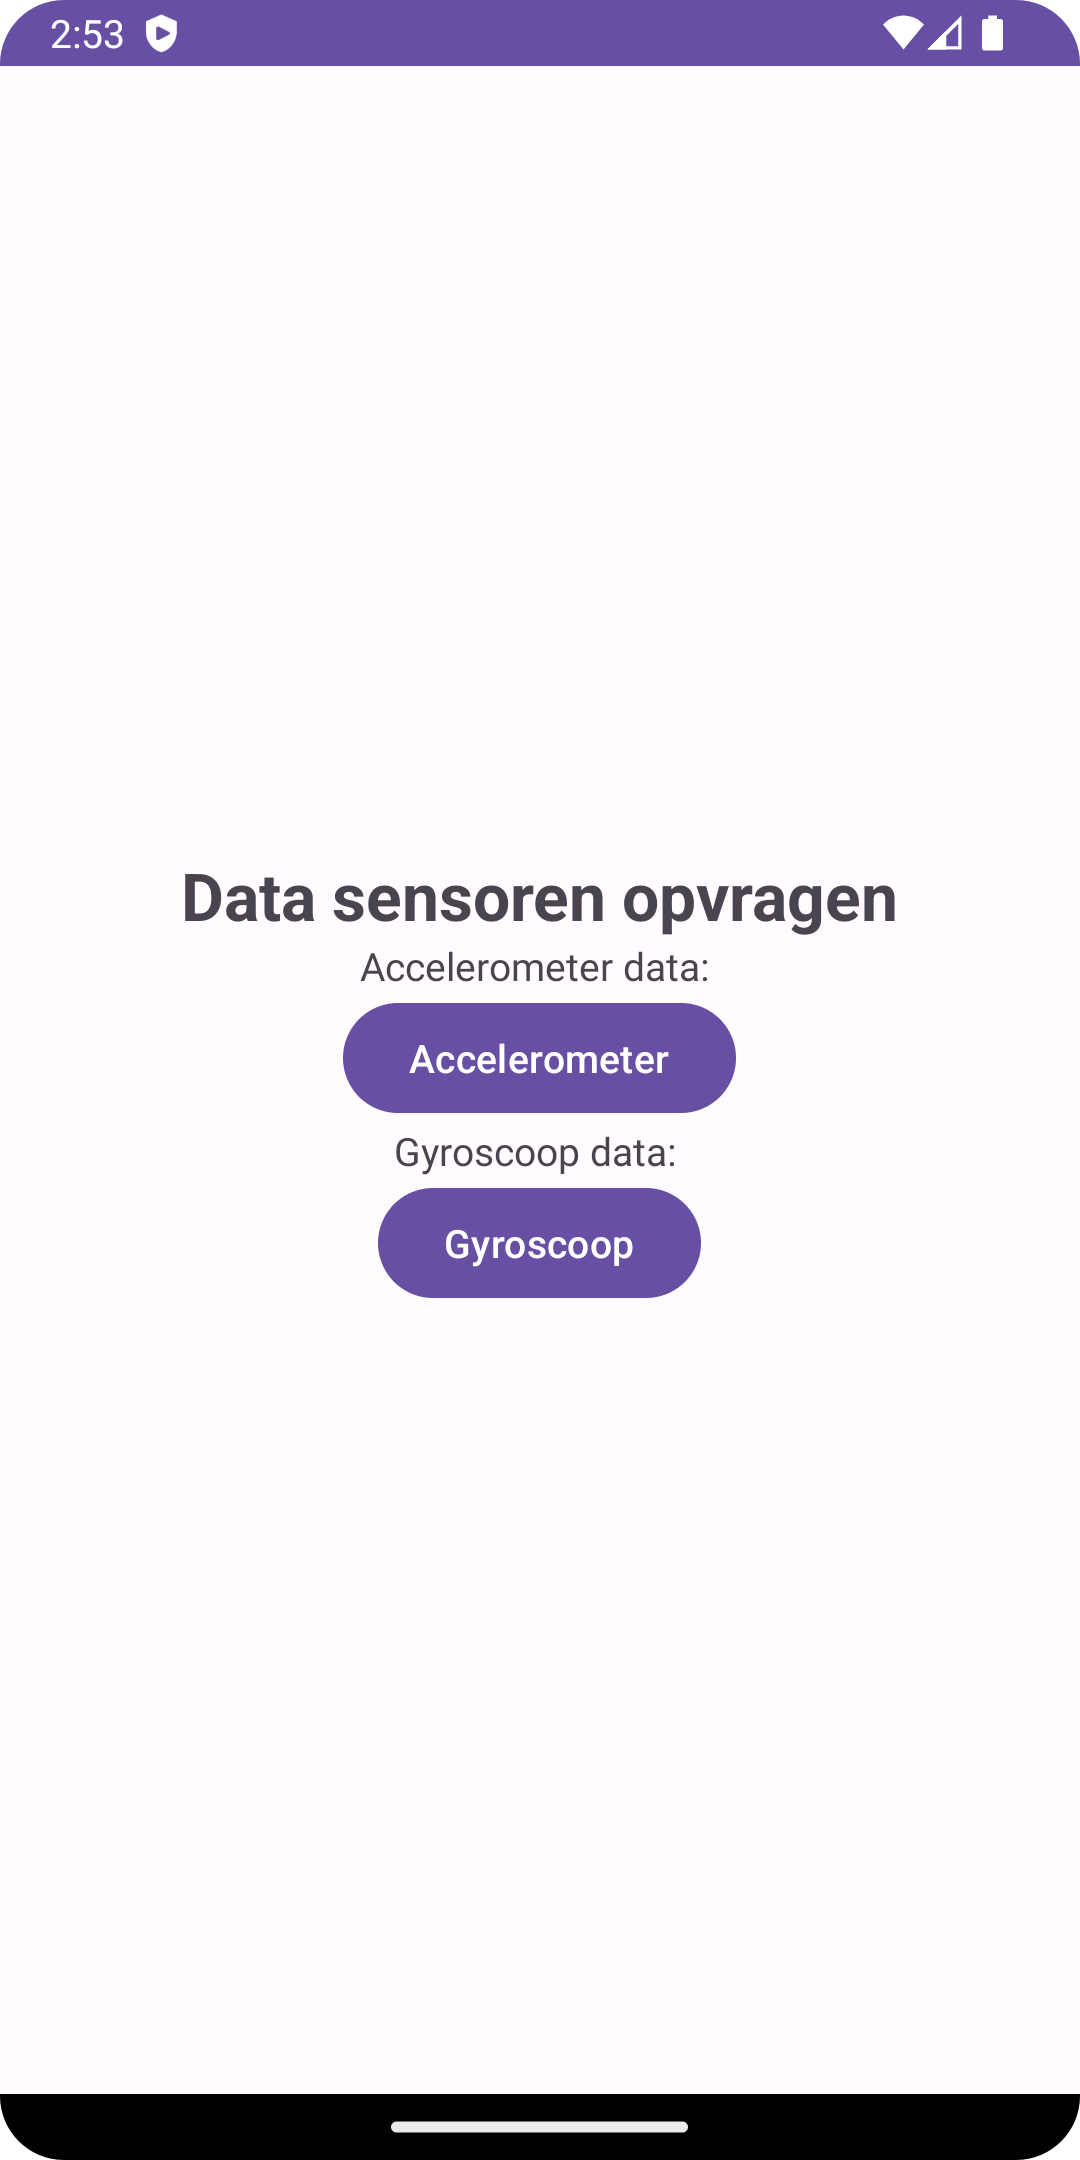
\includegraphics[height=0.5\textheight]{sensoren_layoutnative.png}
    \caption{Layout van applicatie voor data van sensoren op te halen bij Android.}
\end{figure}

\subsubsection{Ontwikkeltijd}

Aangezien dat er geen extra libraries of tools gebruikt worden om de sensoren te gebruiken, 
kunnen de sensoren snel geïmplementeerd worden. Enkel moeten de juiste 
permission worden toegevoegd aan het AndroidManifest.xml bestand, de juiste klasse moet geïmporteerd worden en de juiste 
methode moet worden aangeroepen. Daarom is de tijd nodig om de sensoren te gebruiken dus zeer laag. 
Er is ongeveer 45 minuten gespendeerd om de sensoren te implementeren, inclusief opzoekwerk. Er zijn ook geen grote problemen of 
bugs voorgekomen tijdens de implementatie.




\subsubsection{Performantie}

\paragraph{Tijdsduur}
\begin{figure}[H]
    \centering
    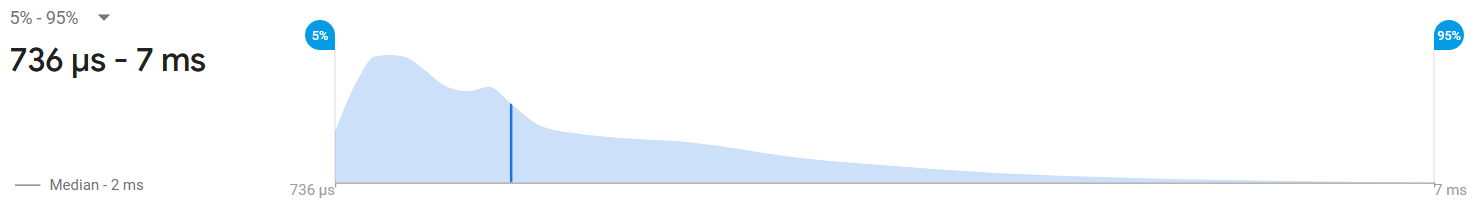
\includegraphics[height=0.085\textheight]{sensorenDuratieNativeAccelerometer.png}
    \caption{Overzicht tijdsduur ophalen van accelerometer data bij Android.}
\end{figure}
Van zodra er op de knop wordt gedrukt om gegevens op te halen van de accelerometer blijft de applicatie
dit continu doen. Hierdoor worden er honderden metingen gedaan die ons vertellen dat het ophalen 
van de accelerometer data gemiddeld 2ms duurt. De minimum en maximum waarden liggen op 736µs en 7ms.
\begin{figure}[H]
    \centering
    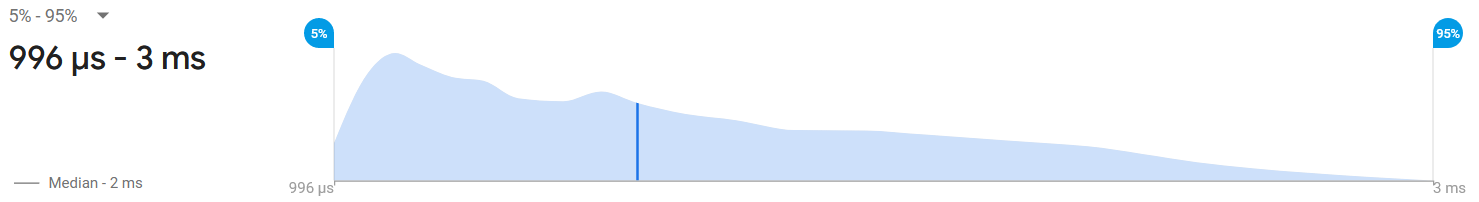
\includegraphics[height=0.085\textheight]{sensorenDuratieNativeGyroscoop.png}
    \caption{Overzicht tijdsduur ophalen van gyroscoop data bij Android.}
\end{figure}
Net zoals bij de accelerometer worden er constant gegevens opgehaald van zodra er op de knop wordt gedrukt. 
Hierdoor worden er opnieuw honderden metingen gedaan die ons vertellen dat het ophalen 
van de gyroscoop data gemiddeld 2ms duurt. De minimum en maximum waarden liggen op 996µs en 3ms.

\paragraph{CPU \& geheugen}
\begin{figure}[H]
    \centering
    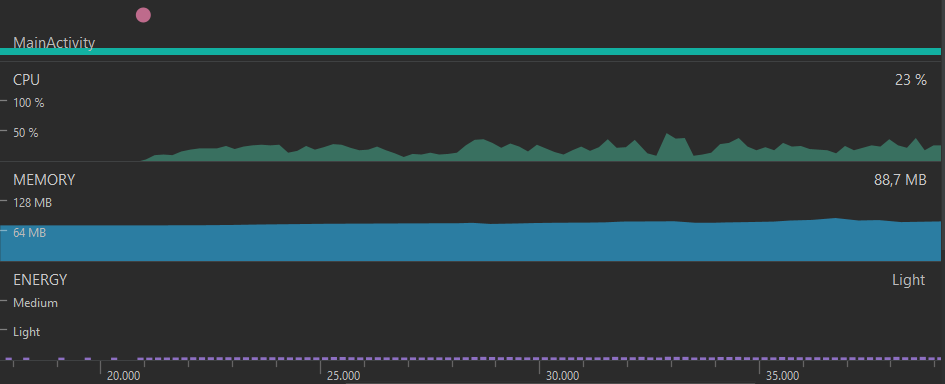
\includegraphics[height=0.25\textheight]{sensorenPerformantieNativeAccelerometer.png}
    \caption{Overzicht CPU en geheugen gebruik tijdens het ophalen van accelerometer data bij Android.}
\end{figure}
Op de grafiek is te zien dat het CPU gebruik van de applicatie bij het ophalen van de accelerometer data,
gemiddeld 23\% is met toch wel redelijke schommelingen. Wanneer er nog geen data wordt opgehaald, wordt de CPU niet 
gebruikt. Het geheugen blijft rond de 88MB hangen, met verschillen van maximum 4-5MB. 
Er is geen merkbaar verschil in het geheugen wanneer er data wordt opgehaald of wanneer er 
geen data wordt opgehaald.
\begin{figure}[H]
    \centering
    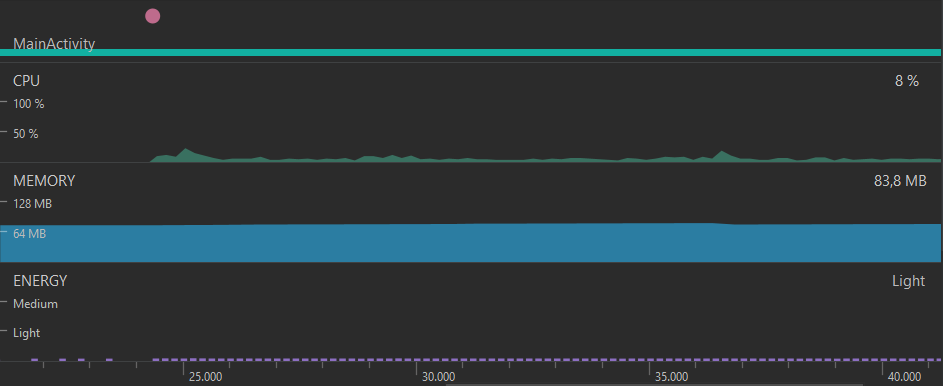
\includegraphics[height=0.25\textheight]{sensorenPerformantieNativeGyroscoop.png}
    \caption{Overzicht CPU en geheugen gebruik tijdens het ophalen van gyroscoop data bij Android.}
\end{figure}
Net zoals bij de accelerometer is op de grafiek te zien dat het CPU gebruik van de applicatie bij het 
ophalen van de gyroscoop data, gemiddeld 8\% is. Wat opvalt, is dat er bij het ophalen van de gyroscoop data
in het begin een piek is van 30\%. Maar dat dit daarna terug zakt naar 8\%. Bij de accelerometer was er geen
piek te zien maar was het gemiddelde CPU gebruik wel hoger. Net zoals bij de accelerometer is er ook geen 
CPU gebruik wanneer er geen data wordt opgehaald. Het geheugen blijft terug rond de 88MB hangen, met 
verschillen van maximum 4-5MB. Opnieuw is er geen merkbaar verschil in het 
geheugen wanneer er data wordt opgehaald of wanneer er geen data wordt opgehaald.
  


\subsubsection{Schaalbaarheid}

\paragraph{Complexiteit}
Het proces om de data van sensoren te verkrijgen is vrij simpel. De ontwikkelaar moet enkel de juiste klasse importeren, 
de juiste methode aanroepen en de juiste permissies toevoegen aan de AndroidManifest.xml file. Indien dat er iets niet 
duidelijk is, is er altijd de documentatie van Android waarin alles duidelijk wordt uitgelegd.

\paragraph{Herbruikbaarheid}
Het is gemakkelijk om de gegevens van de sensoren te hergebruiken. We kunnen bijvoorbeeld in plaats van de 
gegevens in een TextView component te tonen, de gegevens in een object opslaan. Dat object kan dan vanuit 
een andere klasse worden opgevraagd. Het is ook mogelijk om de logica voor het ophalen van de gegevens
in een aparte klasse te plaatsen. Zo kan de logica gemakkelijk worden hergebruikt in andere klassen. 
En kan deze ook aangepast of opgeschaald worden.



\section{Cross-platform}
\subsubsection{Wat hebben we nodig}
Om bij React Native toegang te krijgen tot de sensoren moet er gebruik worden gemaakt van de react-native-sensors library.
Deze library biedt onder andere toegang tot de accelerometer en gyroscoop. Het is een wrapper voor de
native sensoren van Android en iOS. 

\subsubsection{Uitvoering}

\paragraph{1. Library toevoegen}
Als eerst voegen we React Native Sensors toe aan de root van ons project.
\begin{minted}{bash}
npm install react-native-sensors --save
\end{minted}

\paragraph{2. Package teruggeven}
Normaal gezien moeten we de package dan toevoegen aan het 
\textit{android/app/src/} \textbf{main/java/com/project/MainApplication.java} bestand.
Maar dit is niet meer nodig bij React Native 0.60+.

\paragraph{3. gradle instellingen aanpassen}
Tot slot voegen we de volgende regel toe aan het \textit{android/app/build.gradle} bestand.
\begin{minted}{groovy}
implementation project(':react-native-sensors')
\end{minted}
En voegen we de volgende regel toe aan het \textit{android/settings.gradle} bestand.
\begin{minted}{groovy}
include ':react-native-sensors'
project(':react-native-sensors').projectDir = 
    new File(rootProject.projectDir
        , '../node_modules/react-native-sensors/android')
\end{minted}
De package is nu volledig geïnstalleerd en klaar voor gebruik.

\paragraph{4. Sensor gebruiken}
Eerst importeren we de library in het bestand waar we deze nodig hebben.
\begin{minted}{typescript}
import { accelerometer, gyroscope } from "react-native-sensors";
\end{minted}
Daarna definiëren we twee variabelen die de data van de sensoren zal bewaren.
\begin{minted}{typescript}
const [accelerometerData, setAccelerometerData] = useState({});
const [gyroscopeData, setGyroscopeData] = useState({});
\end{minted}
Tot slot kunnen we dan deze variabelen gebruiken om de data van de sensoren op te vragen.
\begin{minted}{typescript}
const getData = () => {
    setIsFetchingData(true);

    startFetchingData();
};

const startFetchingData = () => {
    if (isFetchingData) {
        const accelerometerSubscription = new Accelerometer({
            updateInterval: 100, // Verander dit indien nodig
        }).subscribe(({ x, y, z }) => {
            // Doe iets met de accelerometerwaarden (x, y, z)
        });

        const gyroscopeSubscription = new Gyroscope({
        updateInterval: 100, // Verander dit indien nodig
        }).subscribe(({ x, y, z }) => {
            // Doe iets met de accelerometerwaarden (x, y, z)
        });

        // Unsubscribe van de sensoren wanneer je klaar bent 
        // met het ophalen van de data
        return () => {
            accelerometerSubscription.unsubscribe();
            gyroscopeSubscription.unsubscribe();
        };
    }
};
\end{minted}

\paragraph{4. Applicatie maken}
Net zoals bij de native applicatie maken we een applicatie die de accelerometer en gyroscoop data 
opvraagt en weergeeft. Deze bestaat uit twee \textbf{<Text>} componenten voor de data van de
accelerometer en gyroscoop weer te geven en tot slot twee \textbf{<Button>} componenten om de 
data op te halen. Als de knoppen ingedrukt worden, dan wordt ofwel de
\textbf{onPress} of \textbf{onPress} methode aangeroepen. In deze methodes wordt de data 
van de sensoren opgehaald en in de \textbf{<Text>} componenten geplaatst.
\begin{figure}[H]
    \centering
    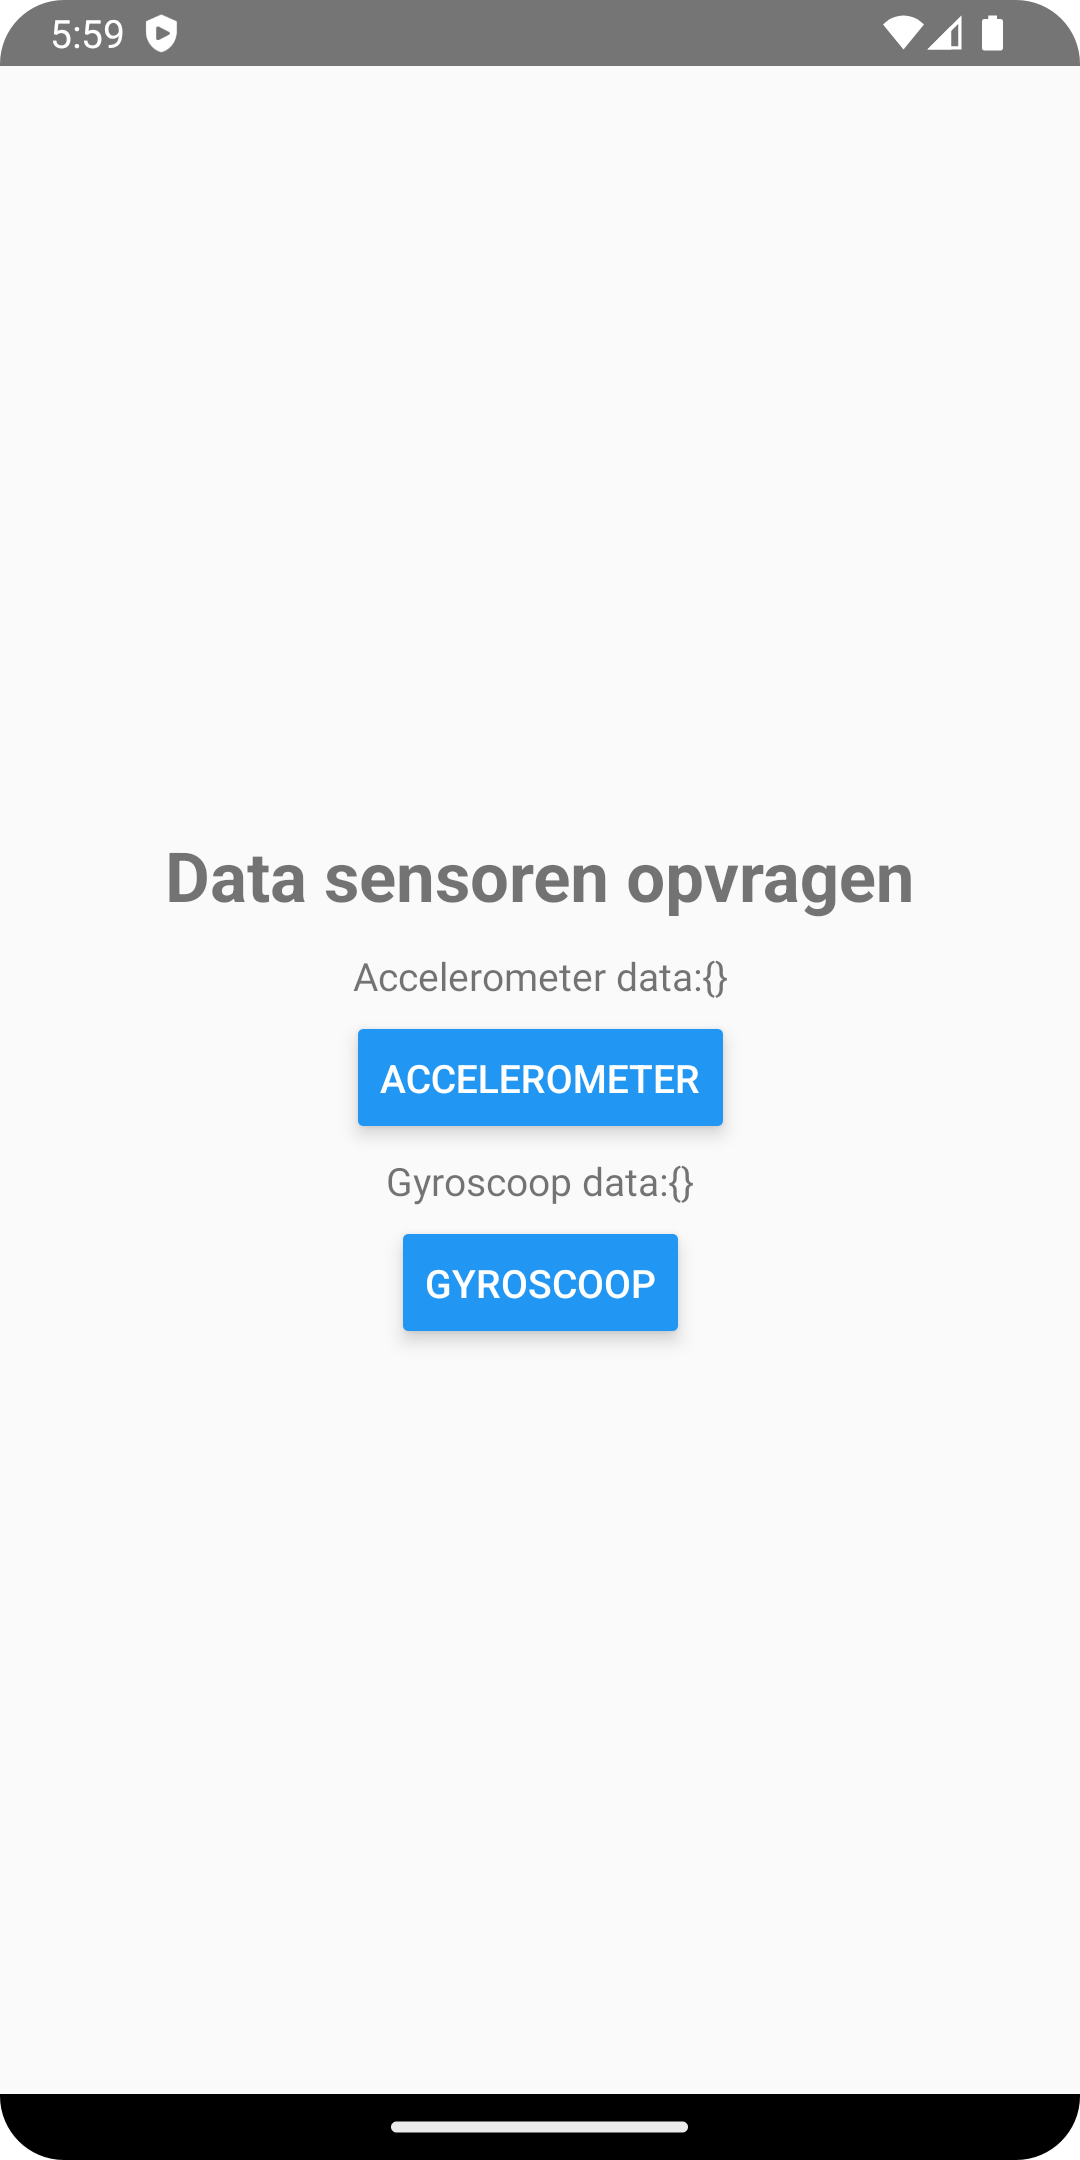
\includegraphics[height=0.4\textheight]{sensoren_layoutcross.png}
    \caption{Layout van applicatie voor data van sensoren op te halen bij React Native.}
\end{figure}

\subsubsection{Ontwikkeltijd}

In vergelijking met native ontwikkeling, moeten er wel meer stappen ondernomen worden om de 
sensoren te gebruiken. Eerst en vooral moet er een externe library geïmplementeerd worden 
om de sensoren te gebruiken. Pas daarna kunnen de sensoren worden gebruikt. Daardoor is de tijd die nodig
was om de sensoren te gebruiken hoger dan bij native ontwikkeling. We hebben ongeveer
1 uur en 15 minuten gespendeerd om de sensoren te gebruiken. Er zijn ook geen grote problemen of
bugs voorgekomen tijdens de implementatie.


\subsubsection{Performantie}

\paragraph{Tijdsduur}
\begin{figure}[H]
    \centering
    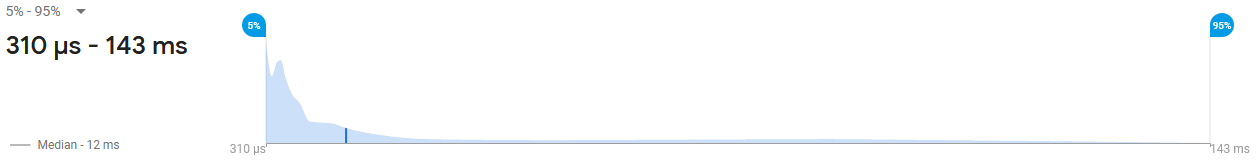
\includegraphics[height=0.1\textheight]{sensorenDuratieCrossAccelerometer.png}
    \caption{Overzicht tijdsduur ophalen van accelerometer data bij React native.}
\end{figure}


\begin{figure}[H]
    \centering
    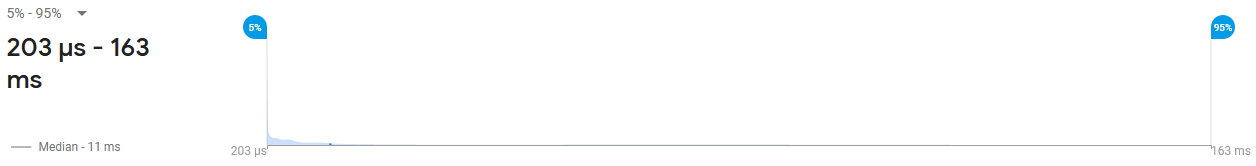
\includegraphics[height=0.1\textheight]{sensorenDuratieCrossGyroscoop.png}
    \caption{Overzicht tijdsduur ophalen van gyroscoop data bij React native.}
\end{figure}


\paragraph{CPU \& geheugen}
\begin{figure}[H]
    \centering
    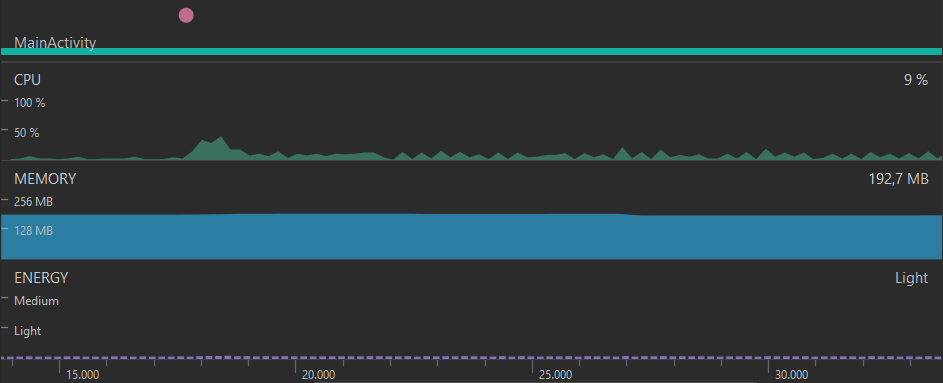
\includegraphics[height=0.3\textheight]{sensorenPerformantieCrossAccelerometer.png}
    \caption{Overzicht CPU en geheugen gebruik tijdens het ophalen van accelerometer data bij React native.}
\end{figure}


\begin{figure}[H]
    \centering
    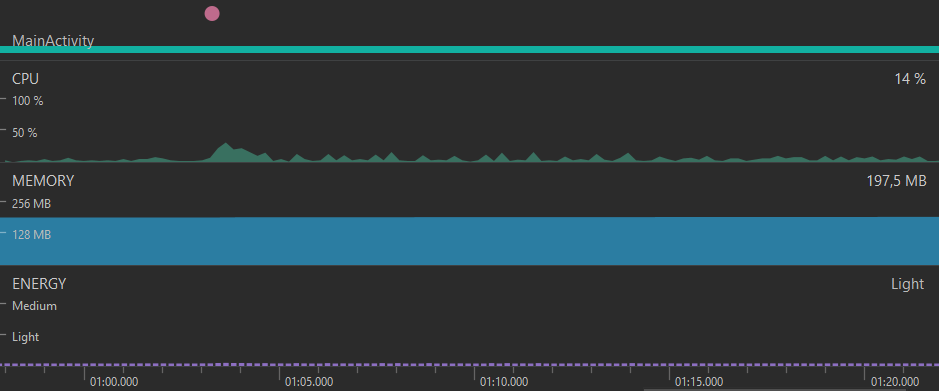
\includegraphics[height=0.3\textheight]{sensorenPerformantieCrossGyroscoop.png}
    \caption{Overzicht CPU en geheugen gebruik tijdens het ophalen van gyroscoop data bij React native.}
\end{figure}


\subsubsection{Schaalbaarheid}

\paragraph{Complexiteit}
Het gebruiken van de sensoren is net zoals bij native vrij simpel. Ondanks dat er een extra library moet worden
geïmplementeerd. De package zorgt ervoor dat het ophalen van de data van de sensoren overeenkomt met het 
ophalen van de data van de sensoren bij native. Daarnaast is er ook net zoals bij native de documentatie van
de library die alles duidelijk uitlegt.

\paragraph{Herbruikbaarheid}
Net zoals bij native is het makkelijk om de gegevens van de sensoren te hergebruiken. We kunnen bijvoorbeeld in plaats van de
gegevens in een useState hook te plaatsen, de gegevens in een globale variabel of in een useContext opslaan. 
Om dan in andere componenten de gegevens op te vragen. Het is ook mogelijk om de logica voor het ophalen van de gegevens
in een aparte useContext te plaatsen. Zo kan de logica makkelijk worden hergebruikt in andere componenten.
En kan deze ook aangepast of opgeschaald worden. 



\section{Conclusie}
Dankzij de resultaten van beide applicaties kunnen we concluderen dat de ontwikkeltijd van het gebruik van sensoren
bij native en cross-platform ongeveer hetzelfde is. Buiten het feit dat we bij cross-platform een extra library moeten
implementeren waardoor de ontwikkeltijd iets langer kan zijn. Bij beide applicaties is er een knop om de methode aan 
te roepen om het ophalen van data te starten.

\begin{tabular}{ |p{3cm}||p{5cm}|p{5cm}| }
    \hline
    \multicolumn{3}{|c|}{Accelerometer} \\ 
    \hline
     & Native (Android) & Cross-platform (React Native) \\
    \hline
     & \multicolumn{2}{|c|}{Tijdsduur} \\
    \hline
    Minimaal & 736µs & 310µs \\
    Maximaal & 7ms & 143ms \\
    Gemiddeld & 2ms & 12ms \\
    \hline
     & \multicolumn{2}{|c|}{Geheugen} \\ 
    \hline
    Offset & 2-3MB & 3-4MB \\
    Gemiddeld & 88MB & 192MB \\
    \hline
     & \multicolumn{2}{|c|}{CPU} \\
    \hline
    (Begin)Piek & / & 50\% \\
    Offset & 20\% & 10\% \\
    Gemiddeld & 23\% & 9\% \\
    \hline
    \multicolumn{3}{|c|}{Gyroscoop} \\ 
    \hline
     & Native (Android) & Cross-platform (React Native) \\
    \hline
     & \multicolumn{2}{|c|}{Tijdsduur} \\
    \hline
    Minimaal & 996µs & 203µs \\
    Maximaal & 3ms & 163ms \\
    Gemiddeld & 2ms & 11ms \\
    \hline
     & \multicolumn{2}{|c|}{Geheugen} \\ 
    \hline
    Offset & 4-5MB & 3-4MB \\
    Gemiddeld & 88MB & 197MB \\
    \hline
     & \multicolumn{2}{|c|}{CPU} \\
    \hline
    (Begin)Piek & 30\% & 40\% \\
    Offset & 5\% & 10\% \\
    Gemiddeld & 8\% & 10\% \\
    \hline
\end{tabular}
\\\\
De tijdsduur van het ophalen van de data van de sensoren is bij native veel sneller dan bij cross-platform.
Dit komt omdat de library die we gebruiken bij cross-platform een wrapper is voor de native sensoren.
Hierdoor moet de data van de sensoren eerst naar de wrapper gestuurd worden en dan pas naar de applicatie.
Bij native is dit niet het geval. De data van de sensoren wordt rechtstreeks naar de applicatie gestuurd.
Het ophalen van data is daardoor gemiddeld 10ms trager bij cross-platform dan bij native.
\\\\
We zien bij het geheugen dat er geen verschil is tussen het ophalen van sensoren data en wanneer er 
niks gebeurd in de applicatie. Maar ondanks dat er geen invloed is om het ophalen van data bij 
Android en React Native zien we wel dat er 121.59\% meer geheugen wordt gebruikt bij React Native dan 
bij Android (88MB in vergelijking met gemiddeld 195MB). Dit komt omdat we bij cross-platform een extra 
library moeten implementeren. Deze library neemt ook geheugen in beslag.
\\\\
Bij het CPU gebruik zijn er onderling tussen de accelerometer en gyroscoop ook verschillen. Bij native 
heeft de accelerometer geen piek maar blijft deze constant op gemiddeld 23\% CPU gebruik. Bij cross-platform zien we
dat de accelerometer een piek heeft van 50\% CPU gebruik en daarna zakt naar 9\% CPU gebruik, een groot verschil. 
Bij de gyroscoop zien we dat bij native de piek 30\% CPU gebruik is en daarna zakt naar 8\% CPU gebruik. Bij cross-platform
is de piek 40\% CPU gebruik en zakt daarna naar 10\% CPU gebruik. Ook is er bij alle sensoren een schommeling van 5 tot 20\% 
CPU gebruik. Dit komt omdat de sensoren data constant wordt opgehaald. Normaal zou er verwacht worden dat de sensoren bij native 
minder CPU gebruiken, aangezien de data eerst naar de wrapper wordt gestuurd en dan pas naar de applicatie. Maar bij 
de accelerometer is dit niet het geval. Hier is het CPU gebruik bij cross-platform lager dan bij native.
\\\\
Op vlak van schaalbaarheid is er geen verschil tussen native en cross-platform. Beide applicaties kunnen
gemakkelijk uitgebreid worden met extra sensoren en de bestaande logica van de sensoren kan gemakkelijk 
hergebruikt of opgeschaald worden.
\\\\
Uit deze resultaten kunnen we concluderen dat we het gebruik van native boven cross-platform Aangeraden is.
Ondanks dat het CPU gebruik bij de accelerometer beter is bij cross-platform dan bij native, is de tijdsduur
van het ophalen van data bij cross-platform veel trager dan bij native. Bij de gyroscoop is het CPU gebruik en 
tijdsduur wel beter bij native. 















%%=============================================================================
%% Push-notificaties
%%=============================================================================

\chapter{Notificaties}%
\label{ch:notificaties}

In dit hoofdstuk worden de lokale notificaties van native en cross-platform vergeleken met elkaar. 
Met de resultaten kan dan een gepaste conclusie worden gevormd.

\section{Native}
\subsubsection{Wat hebben we nodig}
Om lokale notificaties aan te kunnen maken bij Android wordt de NotificationCompat API aangeboden 
door de Android support library. Deze stelt ons in staat om de titel, tekst, pictogram en andere inhoud van de 
notificatie in te stellen. Notificaties kunnen ook worden ingesteld om speciale acties te ondernemen bij het openen 
van de applicatie via de notificatie. Er kan ook een eventueel een prioriteit worden meegegeven.

\subsubsection{Uitvoering}

\paragraph{1. Dependancy toevoegen}
Normaal zijn bevatten alle projecten gestart met Android Studio de nodige dependancies om de NotificationCompat API
te gebruiken. Maar voor de zekerheid verifiëren we dat onderstaande dependancy er bij zit.
\begin{minted}{java}
  val core_version = "1.6.0"
  dependencies {
      implementation("androidx.core:core-ktx:$core_version")
  }
\end{minted}
Als de dependancy is toegevoegd dan kunnen we notificaties beginnen aanmaken.

\paragraph{2. Notificatie aanmaken}
Om een notificatie aan te maken gaan we het NotificationCompat.Builder object gebruiken. 
\begin{minted}{kotlin}
  private fun createNotification(title: String, body: String) {
    val builder = NotificationCompat.Builder(this, CHANNEL_ID)
      .setSmallIcon(icon)
      .setContentTitle(title)
      .setContentText(body)
      .setPriority(NotificationCompat.PRIORITY_DEFAULT)

    val notificationManager: NotificationManager =
      getSystemService(Context.NOTIFICATION_SERVICE) as NotificationManager
    notificationManager.notify(notificationId, builder.build())
}
\end{minted}
\begin{figure}[H]
    \centering
    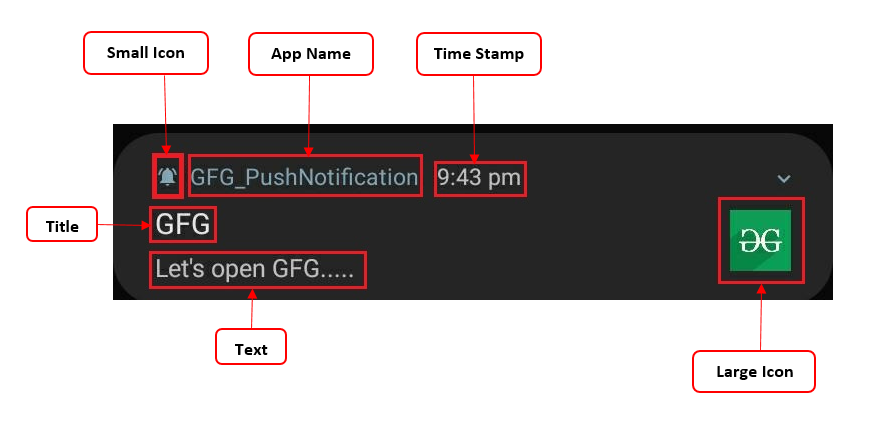
\includegraphics[height=0.3\textheight]{NotificationAnatomy.png}
    \caption{Anatomy standaard notificatie \parencite{One2020}.}
\end{figure}

\paragraph{3. Channel aanmaken}
Het laatste dat we nodig hebben vooraleer de notificatie getoond kan worden is een channel. Deze worden 
gebruikt om notificaties te groeperen volgens hun belang. Om een channel aan te maken gebruiken we 
de .createNotificationChannel() methode. Het maakt niet uit wanneer of waar deze code wordt uitgevoerd. 
Het is enkel belangrijk dat de channel wordt aangemaakt vooraleer er wordt geprobeerd om notificaties 
te tonen. Dus best zo vroeg mogelijk in de applicatie.
\begin{minted}{kotlin}
private fun createNotificationChannel() {
  if (Build.VERSION.SDK_INT >= Build.VERSION_CODES.O) {
    val name = "bachproef"
    val descriptionText = "bachproef notificaties"
    val importance = NotificationManager.IMPORTANCE_DEFAULT
    val channel = NotificationChannel(CHANNEL_ID, name, importance).apply {
      description = descriptionText
    }
    // Channel bij het systeem registreren
    val notificationManager: NotificationManager =
      getSystemService(Context.NOTIFICATION_SERVICE) as NotificationManager
    notificationManager.createNotificationChannel(channel)
  }
}
\end{minted}

\paragraph{4. Applicatie maken}
Met deze informatie kunnen we nu een applicatie opbouwen die notificaties zal sturen. De applicatie bestaat 
uit twee \textbf{EditText} componenten voor een titel en beschijving van de notificatie en tot slot een 
\textbf{Button} om de notificatie te triggeren. Als de knop wordt ingedrukt dan wordt de 
\textbf{createNotification} methode aangeroepen en wordt de waarde van de inputs meegegeven.
\begin{figure}[H]
  \centering
  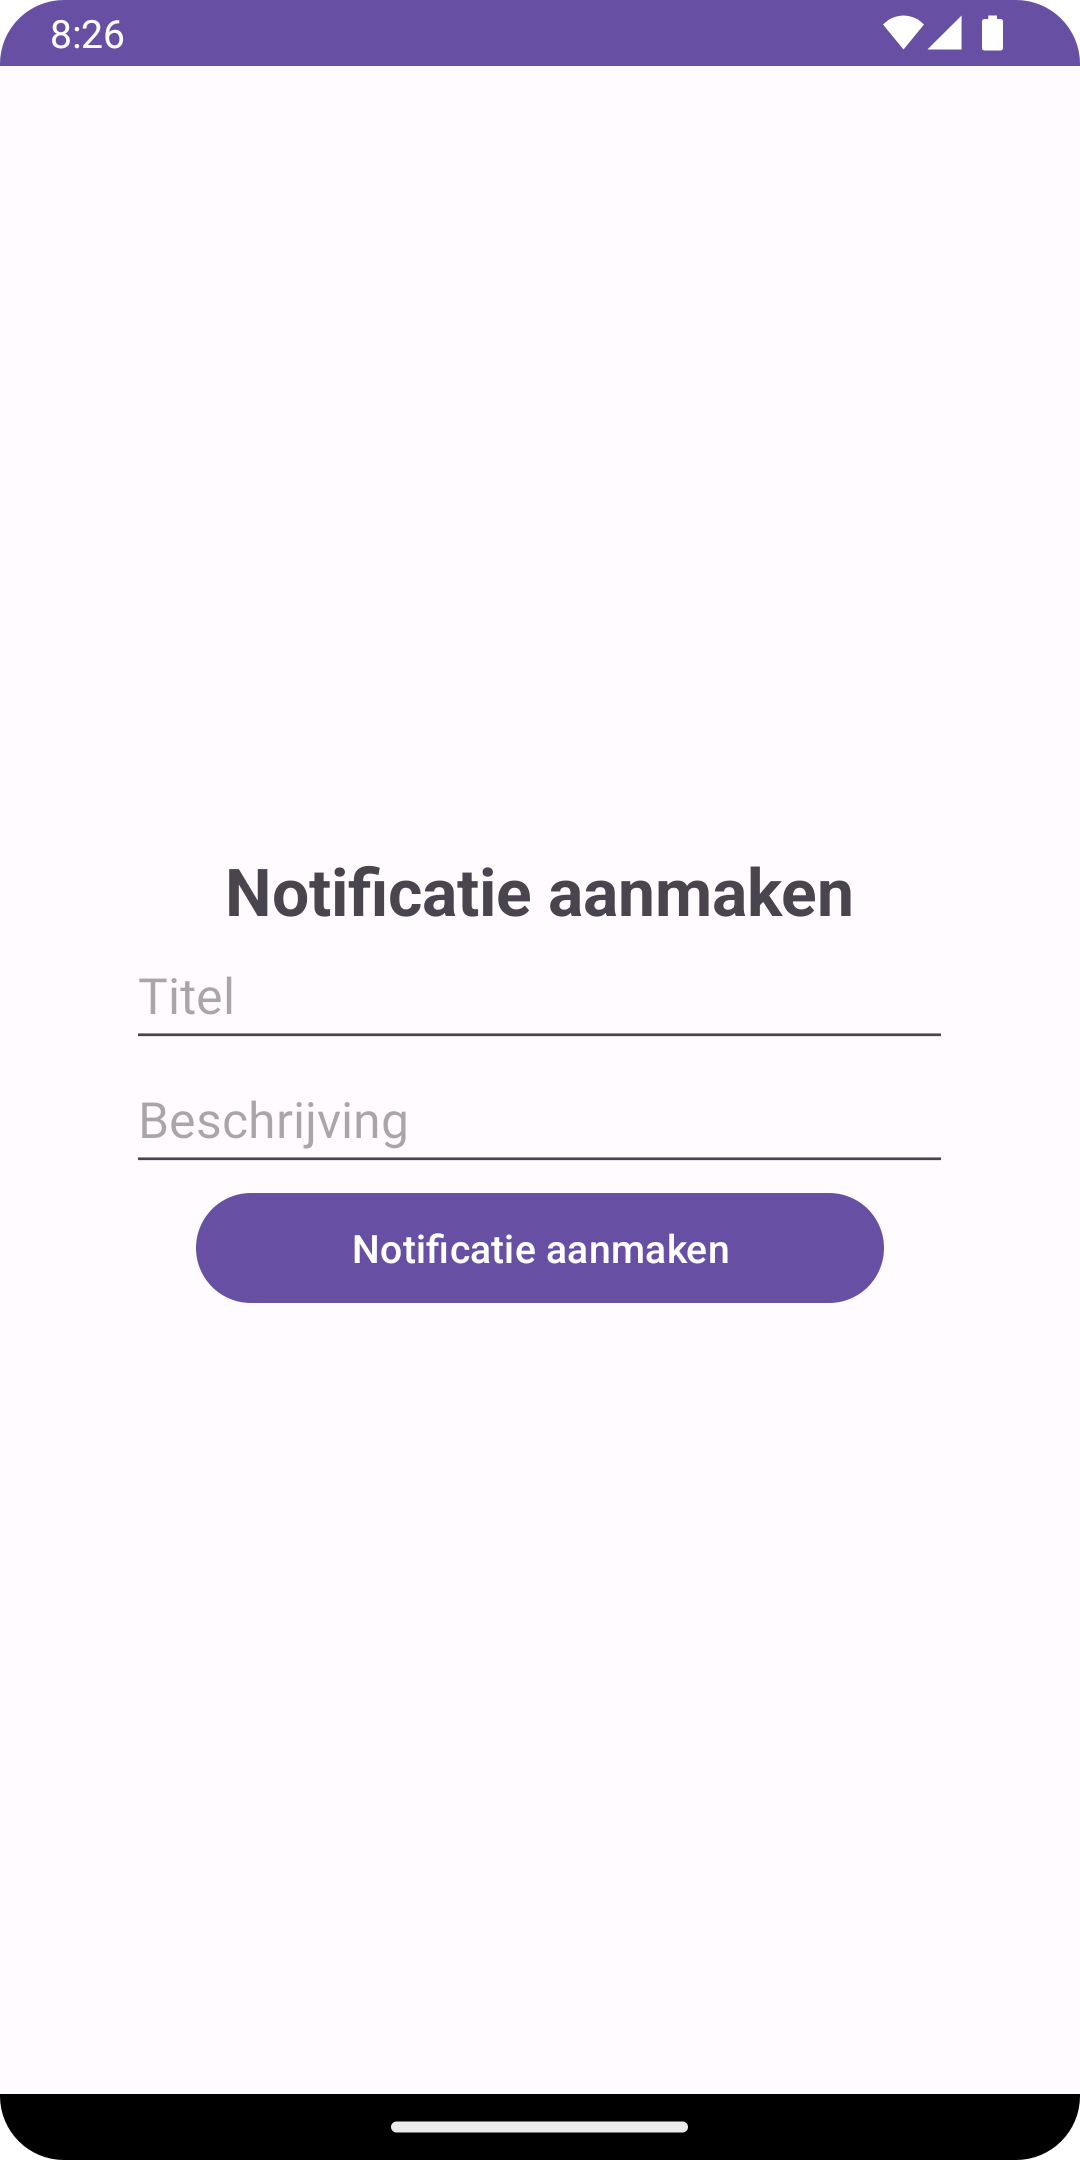
\includegraphics[height=0.5\textheight]{notificaties_layoutnative.png}
  \caption{Layout van applicatie voor notificaties te sturen bij Android.}
\end{figure}

\subsubsection{Ontwikkeltijd}

Ondanks dat er een probleem heeft opgedaan bij het implementeren van de functionaliteit, was 
het implementeren van de notificaties vrij simpel. Als de tijdsduur van het probleem niet wordt meegerekend 
dan kostte het 1 uur en 15 minuten om notificaties te sturen.

\paragraph{Problemen}
Naast de tijd die nodig was om de functionaliteit te implementeren is er ook 2 uur verloren aan een probleem. 
Waarom het probleem zich voordeed is niet duidelijk maar de applicatie vroeg ondanks dat de 
\textbf{POST\_NOTIFICATIONS} bij user-permissions in het AndroidManifest.xml bestand stond 
niet om toestemming om notificaties te sturen. Hierdoor leek het alsof er geen notificaties werden aangemaakt
terwijl het probleem was dat de applicatie geen toestemming had gegeven om notificaties te ontvangen.

\subsubsection{Performantie}

\paragraph{Tijdsduur}
\begin{figure}[H]
    \centering
    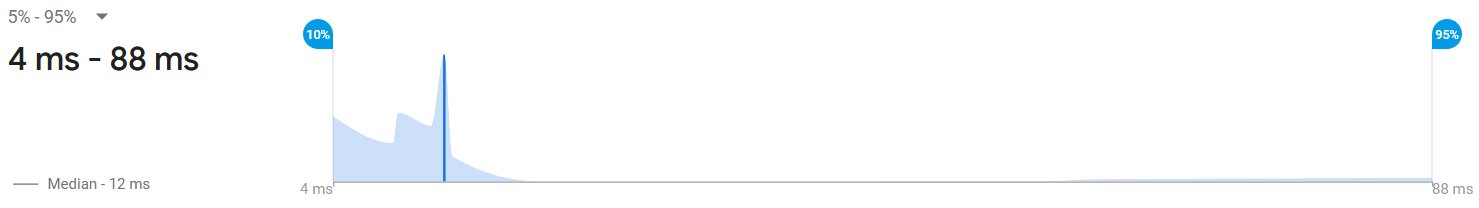
\includegraphics[height=0.1\textheight]{notificatiesDuratieNative.png}
    \caption{Overzicht tijdsduur aanmaken notificaties bij Android.}
\end{figure}
Tijdens het meten van de duur voor het aanmaken van een notificatie, is er 
10 keer een notificatie aangemaakt. Na 10 keer een notificatie aan te maken is er  
een gemiddelde duur van 12ms en met een minimum en 
maximum van 4ms en 88ms.

\paragraph{CPU \& geheugen}
\begin{figure}[H]
    \centering
    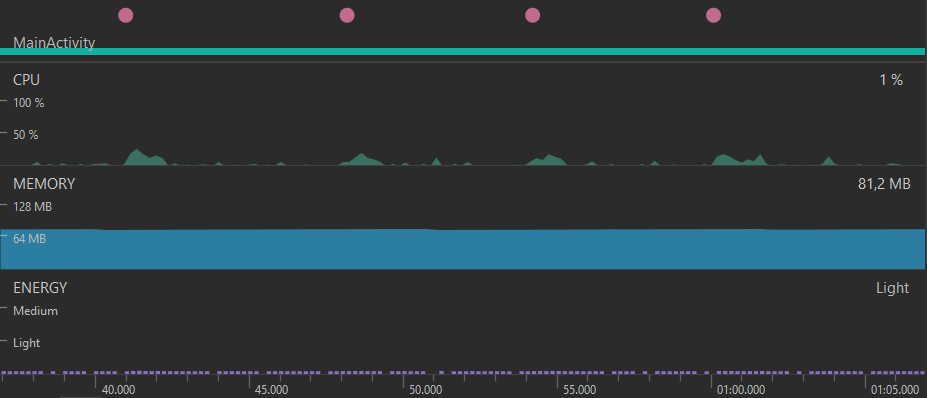
\includegraphics[height=0.25\textheight]{notificatiesPerformantieNative.png}
    \caption{Overzicht CPU en geheugen gebruik tijdens aanmaken notificaties bij Android.}
\end{figure}
Op de grafiek is te zien dat het CPU gebruik van de applicatie wanneer deze inactief is, rond de 4\% ligt. 
Het is ook duidelijk zichtbaar wanneer een notificatie wordt aangemaakt. De piek van het CPU gebruik lag 
gemiddeld op 21\% en schommelde tussen de 19\% en 27\%. Het geheugen blijft in tegenstelling met de CPU 
wanneer de applicatie inactief en actief is, rond de 81MB hangen, met verschillen van maximum 2-3MB. Er is geen 
merkbaar verschil in het geheugen wanneer een notificatie wordt aangemaakt.
  

\subsubsection{Schaalbaarheid}

\paragraph{Complexiteit}
De NotificationCompat API die Android aanbiedt is gemakkelijk om te gebruiken. 
Er moeten normaal gezien geen extra stappen ondernomen worden om de notificaties 
te gebruiken.

\paragraph{Herbruikbaarheid}
het is mogelijk om alle delen van de logica weg te steken in methodes. Op die manier 
is het gemakkelijk om de notificaties later uit te breiden door bijvoorbeeld meerdere channels aan te maken
of op andere plaatsen in het programma een notificatie aan te maken. Het is daardoor ook gemakkelijk om de 
bestaande logica van een notificatie aan te maken te wijzigen aangezien deze allemaal op 1 plaats staan.

\clearpage
\section{Cross-platform}
\subsubsection{Wat hebben we nodig}
Om lokale notificaties bij React Native te tonen wordt de library Notifee gebruikt.
Deze library geeft ons toegang om net zoals bij Android de titel, tekst, pictogram en 
andere inhoud van de notificatie in te stellen. Daarnaast kunnen er ook speciale acties 
of prioriteiten worden ingesteld.

\subsubsection{Uitvoering}

\paragraph{1. Library toevoegen}
Eerst moet de Notifee library aan de root van ons project worden toegevoegd. 
Deze wordt toegevoegd met volgend commando:
\begin{minted}{bash}
npm install --save @notifee/react-native
\end{minted}

\paragraph{2. Toestemming vragen \& channel aanmaken}
Nog voor een notificatie kan getoond worden, moet er eerst toestemming worden gevraagd. 
Aangezien dit bij React Native niet automatisch gebeurt zoals bij Android moet de 
toestemming programmatisch gevraagd worden. Daarnaast zal ook een channel moeten aangemaakt worden.
Net zoals bij Android maakt het niet uit wanneer dit gebeurt maar het moet wel gebeuren 
voordat er notificaties worden gestuurd. Dus best zo vroeg mogelijk in de applicatie.
\begin{minted}{javascript}
export const notificationsSetup = async () => {
  const PERMISSION = await notifee.requestPermission();

  if(PERMISSION.authorizationStatus === AuthorizationStatus.DENIED) {
    return;
  }

  await notifee.createChannel({
    id: 'bachproef',
    name: 'BachproefNotificaties',
  });
}

\end{minted}

\paragraph{3. Notificatie aanmaken}
Bij React Native worden notificaties direct getoond bij het maken ervan. Net zoals bij Android 
wordt er een naam, description, channelId en optioneel een icoon (default ic\_launcher) meegegeven. 
\begin{minted}{javascript}
export const createNotification = async (title: string, body: string) => {
  await notifee.displayNotification({
    title,
    body,
    android: {
      channelId: 'bachproef',
      pressAction: {
        id: 'default',
      },
    },
  });
}
\end{minted}

\paragraph{4. Applicatie maken}
Net zoals bij native zal de applicatie bestaan 
uit twee \textbf{<TextInput/>} componenten voor een titel en beschijving van de notificatie en tot slot een 
\textbf{<Button/>} om de notificatie te triggeren. Als de knop wordt ingedrukt dan wordt de 
\textbf{createNotification} methode aangeroepen en wordt de waarde van de inputs meegegeven.
\begin{figure}[H]
  \centering
  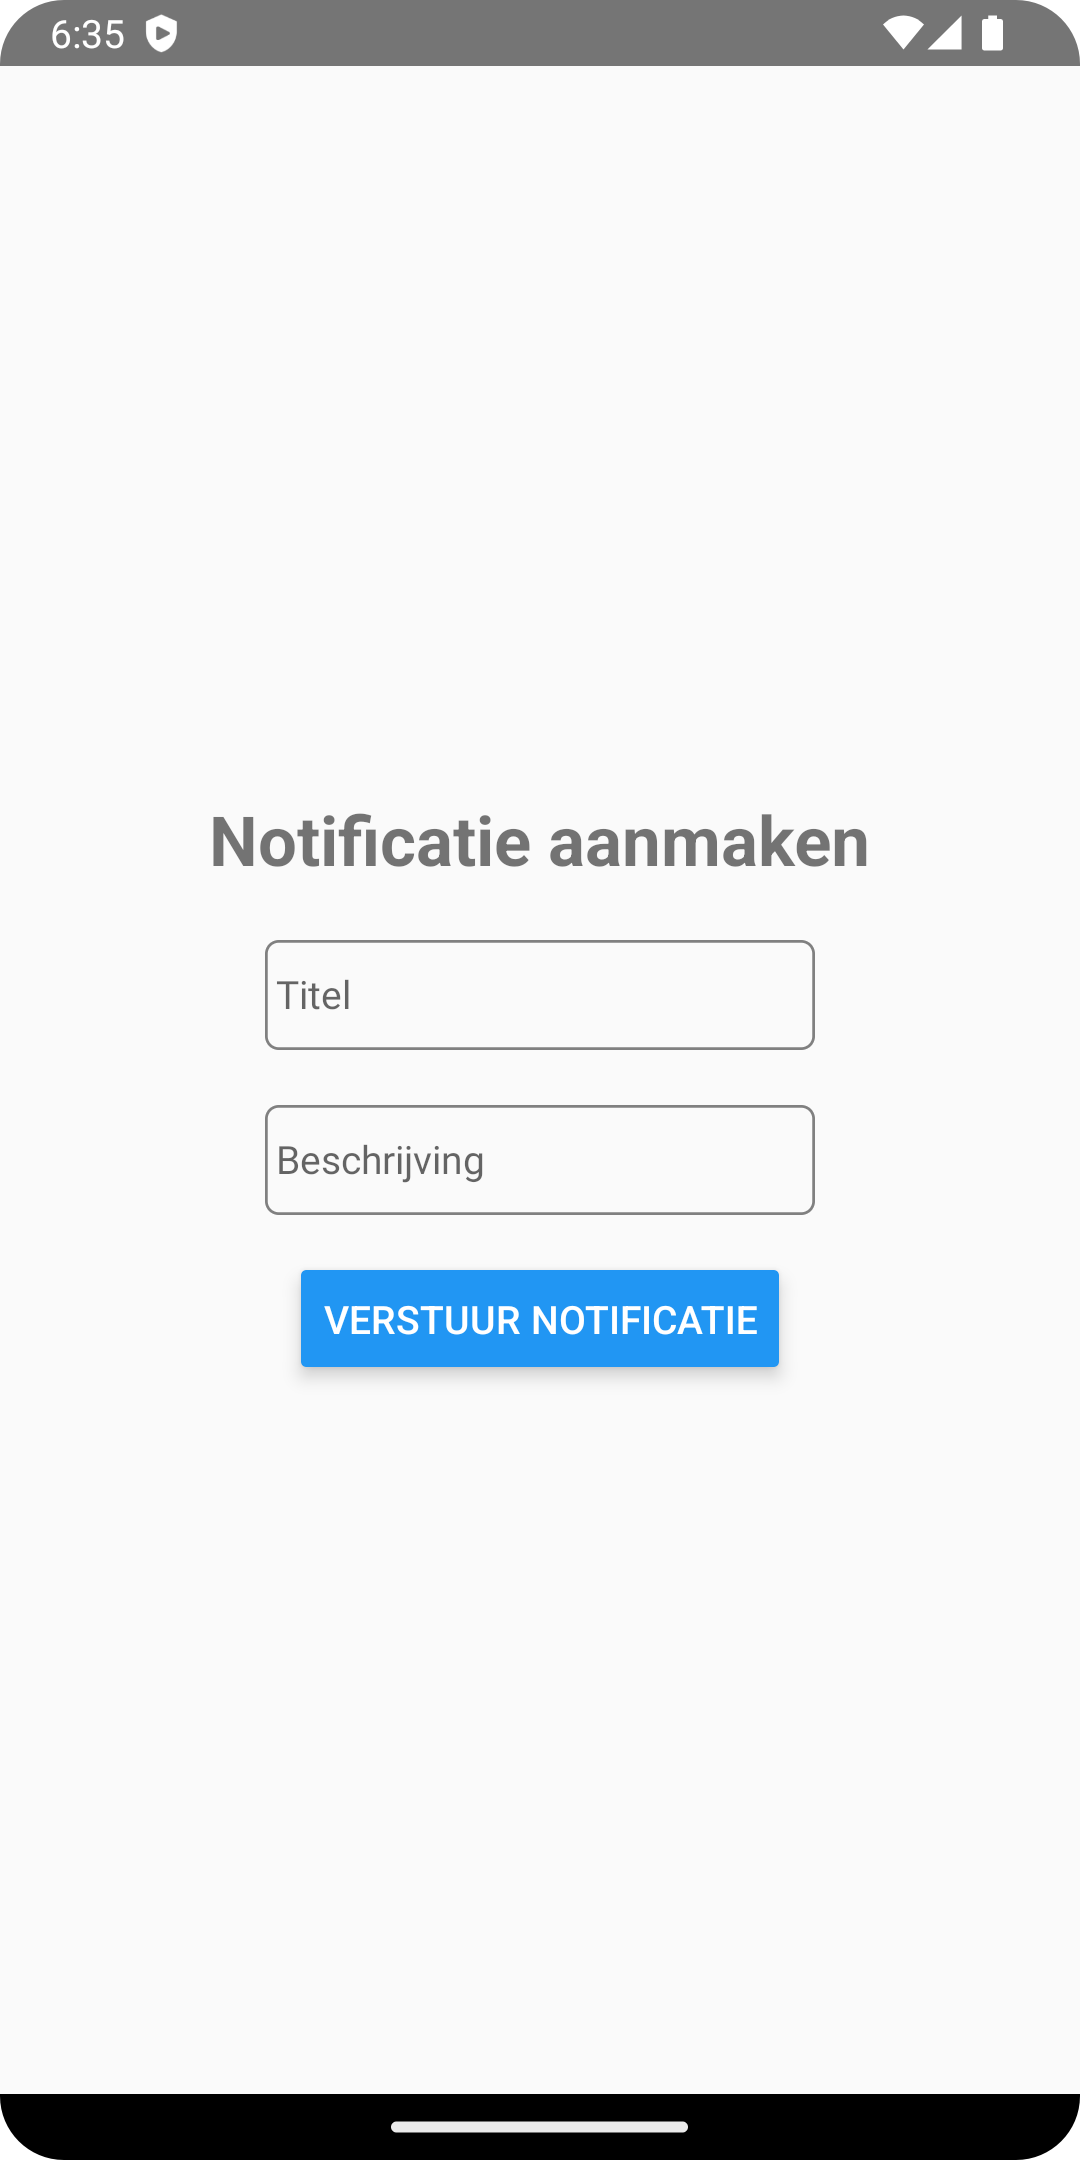
\includegraphics[height=0.5\textheight]{notificaties_layoutcross.png}
  \caption{Layout van applicatie voor notificaties te sturen bij React Native.}
\end{figure}

\subsubsection{Ontwikkeltijd}

Ondanks dat er een externe library gebruikt en geïmplementeerd moest worden, was het implementeren van de 
notificaties functionaliteit zeer simpel. Door gebruik te maken van de documentatie was het mogelijk om 
notificaties te sturen na 1 uur werk. Er zijn ook geen grote problemen of bugs voorgekomen tijdens de implementatie.



\subsubsection{Performantie}

\paragraph{Tijdsduur}
\begin{figure}[H]
  \centering
  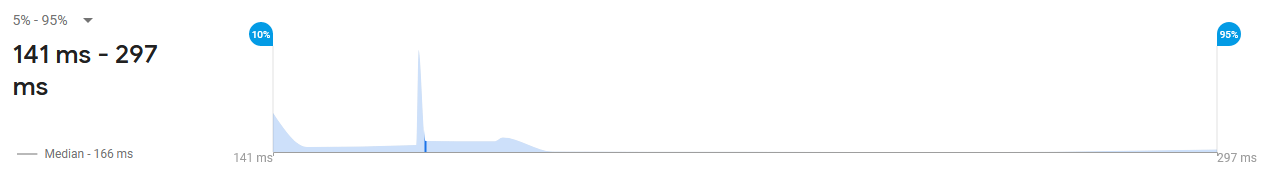
\includegraphics[height=0.085\textheight]{notificatiesDuratieCross.png}
  \caption{Overzicht tijdsduur aanmaken notificaties bij React Native.}
\end{figure}
Tijdens het meten van de duur voor het aanmaken van een notificatie, is er net zoals bij native 
10 keer een notificatie aangemaakt. Na 10 keer een notificatie aan te maken is er 
een gemiddelde duur van 166ms en met een minimum en 
maximum van 141ms en 297ms voor het aanmaken van een notificatie.

\paragraph{CPU \& geheugen}
\begin{figure}[H]
  \centering
  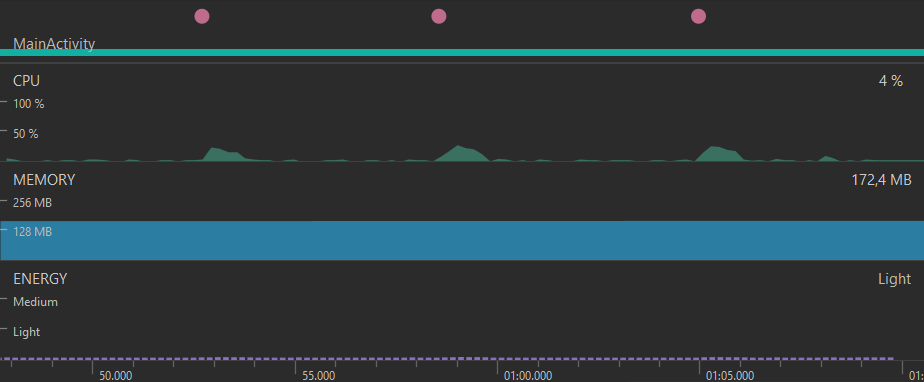
\includegraphics[height=0.25\textheight]{notificatiesPerformantieCross.png}
  \caption{Overzicht CPU en geheugen gebruik tijdens aanmaken notificaties bij React Native.}
\end{figure}
Op de grafiek is te zien dat het CPU gebruik van de applicatie wanneer deze inactief is, rond de 4\% ligt. 
Daarnaast is het duidelijk zichtbaar wanneer een notificatie wordt aangemaakt. De piek van het CPU gebruik lag 
gemiddeld op 28\% en schommelde tussen de 25\% en 30\%. Het geheugen blijft in tegenstelling tot de CPU 
wanneer de applicatie inactief en actief is, rond de 172MB hangen, met verschillen van maximum 0,5MB. 
Er is geen merkbaar verschil in het geheugen wanneer een notificatie wordt aangemaakt.


\subsubsection{Schaalbaarheid}

\paragraph{Complexiteit}
De complexiteit van de library valt goed mee, dankzij de beschikbare documentatie van de library is het zeer 
gemakkelijk om alle mogelijkheden van de library terug te vinden en zelf in een project te implementeren. 

\paragraph{Herbruikbaarheid}
\begin{figure}[H]
    \centering
    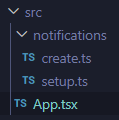
\includegraphics[height=0.1\textheight]{notificationsschaalbaarheidcross.png}
    \caption{Structuur notificaties implementatie React Native.}
\end{figure}
Door de logica van de library op te delen is het gemakkelijk om later opnieuw dezelfde logica op andere plaatsen 
in de code te gebruiken. Er moet enkel een methode geïmporteerd worden om een notificatie aan te maken. Aan die methode 
wordt dan de titel en beschrijving meegegeven. Het is ook mogelijk om de logica voor het aanmaken van een notificatie 
aan te passen. Dit kan dan gemakkelijk gebeuren in het \textbf{create.ts} bestand. Of er kan een nieuwe methode worden 
aangemaakt om bijvoorbeeld de notificatie in te plannen op een later tijdstip.

\section{Conclusie}
Dankzij de resultaten van beide applicaties kunnen we concluderen dat de ontwikkeltijd van notificaties met 
beide ontwikkelmethodes relatief gelijk blijft. Bij beide applicaties moest er toestemming gevraagd worden. 
Door bij Android dit aan het \textbf{AndroidManifest.xml} bestand toe te voegen, en bij React Native door 
de \textbf{notifee.requestPermission();} methode uit te voeren. Hierna moet er bij beide applicaties een 
channel worden aangemaakt en tot slot dan de notificatie.

\begin{tabular}{ |p{3cm}||p{5cm}|p{5cm}| }
    \hline
     & Native (Android) & Cross-platform (React Native) \\
    \hline
     & \multicolumn{2}{|c|}{Tijdsduur} \\
    \hline
    Minimaal & 4ms & 141ms \\
    Maximaal & 88ms & 166ms \\
    Gemiddeld & 12ms & 297ms \\
    \hline
     & \multicolumn{2}{|c|}{Geheugen} \\ 
    \hline
    Offset & 2-3MB & 0,5MB \\
    Gemiddeld & 81MB & 172MB \\
    \hline
     & \multicolumn{2}{|c|}{CPU} \\
    \hline
    Minimaal & 19\% & 25\% \\
    Maximaal & 27\% & 30\% \\
    Gemiddeld & 21\% & 28\% \\
    \hline
\end{tabular}
\\\\
Daarnaast zien we bij de tijdsduur dat nodig is om een notificatie aan te maken wel een duidelijk 
verschil tussen Android en React Native. Gemiddel is het aanmaken van een notificatie bij Android
154ms sneller dan bij React Native. Bij React Native duurt het gemiddel 166ms om een notificatie 
aan te maken terwijl dit bij Android maar 12ms duurt. Dit kan liggen aan het feit dat de externe 
library de code moet omzetten naar platformspecifieke code waardoor er veel tijd wordt verloren.
\\\\
We zien dan wel bij het geheugen dat er geen verschil is tussen het aanmaken van een notificatie en wanneer er 
niks gebeurd in de appplicatie. Maar ondanks dat er geen invloed is om het aanmaken van een notificatie bij 
Android en React Native zien we wel dat er 112,35\% meer geheugen wordt gebruikt bij React Native dan 
bij Android (81MB in vergelijking met 172MB). Dit kan ook weer liggen aan het feit dat de externe library
de code moet omzetten naar platformspecifieke code waardoor er veel geheugen wordt gebruikt.
\\\\
Bij het CPU gebruik zien we wel een verschil tijdens het aanmaken van een notificatie en wanneer de 
applicatie inactief is. Daarnaast zien we ook een verschil tussen Android en React-native. Bij React Native 
springt het CPU gebruik gemiddeld naar 28\% terwijl dat het bij Android maar naar 21\% springt. Ookal 
draaien beide applicaties op hetzelfde apparaat gebruikt de React Native applicatie gemiddeld 7\% meer 
van de CPU dan de Android applicatie.
\\\\
Op vlak van schaalbaarheid merken we dat beide ontwikkelmethodes net zoals bij de ontwikkelingstijd 
lijken op elkaar. Allebei geven ze de mogelijkheid om de logica in methodes te onderscheiden, 
waardoor deze later individueel herbruikt of opgeschaald kunnen worden.
\\\\
Over het algemeen kunnen we concluderen dat het aanmaken van notificaties bij Android sneller gaat dan bij
React Native. En het dus beter is om met native te werken als je notificaties wilt gebruiken in je applicatie.
























%%=============================================================================
%% Audio- en videospelers
%%=============================================================================

\chapter{Audio- en videospelers}%
\label{ch:audioenvideo}

In dit hoofdstuk gaan we de audio- en video mogelijkheden van native en cross-platform vergelijken. Met deze resultaten kunnen we dan een gepaste conclusie vormen.

\section{Native}
\subsubsection{Wat hebben we nodig}
%tools, libraries, ...

\subsubsection{Uitvoering}

\subsubsection{Ontwikkeltijd}

\paragraph{Geïnvesteerde tijd}

\paragraph{Compiletijd}

\subsubsection{Performantie}

\subsubsection{Schaalbaarheid}

\subsubsection{Conclusie}


\section{Cross-platform}
\subsubsection{Wat hebben we nodig}
%tools, libraries, ...

\subsubsection{Uitvoering}

\subsubsection{Ontwikkeltijd}

\paragraph{Geïnvesteerde tijd}

\paragraph{Compiletijd}

\subsubsection{Performantie}

\subsubsection{Schaalbaarheid}

\subsubsection{Conclusie}
























%%=============================================================================
%% Conclusie
%%=============================================================================

\chapter{Conclusie}%
\label{ch:conclusie}

\section{Hoofdonderzoeksvraag}
In dit onderzoek werd er gezocht naar een antwoord op de hoofdonderzoeksvraag:
\begin{itemize}
    \item Hoe verschillen de prestaties, schaalbaarheid en ontwikkeltijd van functionaliteiten tussen native en cross-platform ontwikkeling van mobiele applicaties?
\end{itemize}
Om een antwoord te vinden op deze vraag werden er twee applicaties ontwikkeld, één native en één cross-platform.
Bij deze applicaties werden dan verschillende functionaliteiten geïmplementeerd en is de performantie getest. 
Daarnaast is er ook gekeken naar de ontwikkeltijd en schaalbaarheid van de applicaties. 

\subsection{Ontwikkeltijd}
\subsubsection{Algemene ontwikkeltijd}
Over het algemeen is de ontwikkeltijd bij cross-platform langer dan bij native.
Dit komt door de libraries die geïnstalleerd moeten worden, wat extra tijd in beslag neemt en meer 
ruimte geeft voor fouten. Deze fouten moeten dan ook nog eens opgelost worden, wat ook weer extra tijd in beslag neemt.
\\\\
De ontwikkeltijd is ook langer omdat de React Native libraries de bestaande implementatie van de 
native platformen gebruiken en op verder bouwen. Hierdoor is er soms meer code nodig bij 
cross-platform om dezelfde functionaliteit te krijgen.

\subsubsection{Compiletijd}
De compiletijd bij cross-platform is altijd langer dan bij native. Dit komt omdat er bij cross-platform
een extra stap is bij het compileren. De code wordt eerst gecompileerd naar Javascript, dan pas naar native.
Bij native is er maar één stap, de code wordt gecompileerd naar native.
\\\\
Ondanks het feit dat de compiletijd langer is bij cross-platform, is het niet altijd nodig om de applicatie te compileren.
React Native heeft een hot reload functie, waardoor de applicatie niet gecompileerd moet worden bij het testen.
Eenmaal de applicatie gecompileerd is, kunnen er veranderingen worden aangebracht aan de code en deze worden dan
automatisch doorgevoerd in de applicatie. Dit is een groot voordeel bij het ontwikkelen van de applicatie,
omdat er geen tijd verloren gaat aan het compileren van de applicatie.

\subsection{Performantie}
\subsubsection{Tijdsduur}
Op het vlak van tijdsduur is er enkel een groot verschil bij het aanmaken van notificaties.
Bij cross-platform duurt het aanmaken van een notificatie 14 keer langer dan bij native.
Ook al is dit een groot verschil, het aanmaken van een notificatie duurt bij cross-platform 
nog steeds maar 166ms. Dit is nog steeds snel genoeg om de gebruiker niet te storen 
aangezien dit gebeurt op de achtergrond. Bij de andere functionaliteiten is er wel een verschil
in tijdsduur, maar dit verschil is niet zo groot dat het storend is voor de gebruiker of dat het een 
reden is om cross-platform niet te gebruiken.

\subsubsection{CPU gebruik}
Bij het CPU gebruik zijn de resultaten wisselvallig. Over het algemeen is het CPU gebruik bij cross-platform
hoger dan bij native, maar dit is niet altijd het geval. Bij het gebruik van sensoren bijvoorbeeld is het CPU gebruik
bij cross-platform lager dan bij native. Maar als we dan kijken naar het CPU gebruik bij het afspelen van audio en 
video, dan is het CPU gebruik bij cross-platform hoger dan bij native. Bij het kiezen van een ontwikkelmethode is het 
dus belangrijk om te kijken naar de functionaliteiten die gebruikt zullen worden in de applicatie. 
Deze zullen bepalend zijn voor de uiteindelijke keuze van de ontwikkelmethode.

\subsubsection{Geheugengebruik}
Op het vlak van geheugengebruik is nooit een merkbaar verschil geweest bij het uitvoeren van functionaliteiten 
of wanneer de applicatie inactief is. Daarnaast was het gemiddelde geheugengebruik bij alle functionaliteiten 
bij cross-platform veel hoger dan bij native. Het geheugengebruik bij cross-platform is gemiddeld 2,5 keer hoger
dan bij native. Dit is een groot verschil, als gevolg van de libraries die gebruikt worden bij cross-platform.
Alle extra libraries die gebruikt worden bij cross-platform nemen extra geheugen in beslag. Ook de React 
Native library die altijd standaard is geïnstalleerd, neemt extra geheugen in beslag. Dit is een nadeel bij
cross-platform, maar het is niet zo groot dat het een reden is om cross-platform niet te gebruiken aangezien 
de meeste smartphones tegenwoordig genoeg geheugen hebben om cross-platform applicatie te runnen zonder dat
de gebruiker hier iets van merkt.

\subsection{Schaalbaarheid}
\subsubsection{Complexiteit}
Over het algemeen is de complexiteit gelijkaardig bij native en cross-platform. Bij cross-platform is er wel
meer complexiteit bij het opzetten van de applicatie, maar dit is een eenmalige complexiteit. Er bestaan wel 
complexe libraries bij cross-platform, maar deze zijn niet verplicht om te gebruiken.

\subsubsection{Herbruikbaarheid}
Zowel native als cross-platform hebben een hoge herbruikbaarheid. Bij beide methodes is het mogelijk
om de code te centraliseren en te hergebruiken op andere plaatsen binnen de applicatie of vanop de 
gecentraliseerde plaats de code op te schalen. Het is ook mogelijk om de code te hergebruiken in 
andere applicaties.

\section{Deelonderzoeksvragen}
Naast de hoofdonderzoeksvraag zijn er twee deelonderzoeksvragen waar er een antwoord op gezocht werd 
bij het uitvoeren van dit onderzoek. 
\begin{itemize}
    \item Zijn er functionaliteiten die cross-platform niet ondersteunen?
    \item Zijn er functionaliteiten bij cross-platform waarbij de performantie de functionaliteit onbruikbaar maakt?
\end{itemize}
Bij de vraag of er functionaliteiten zijn die cross-platform niet ondersteunt, 
is er gebleken dat dit niet het geval is. Alle functionaliteiten die in dit onderzoek zijn geïmplementeerd
waren mogelijk bij cross-platform. Bij sommige functionaliteiten had cross-platform meerdere libraries 
die de functionaliteit ondersteunden, terwijl er bij native altijd maar één implementatie mogelijk was.
\\\\
Bij de vraag of er functionaliteiten onbruikbaar zijn bij cross-platform ontwikkeling vanwege de performantie, 
is de conclusie getrokken dat dit niet het geval is. Alle functionaliteiten die in dit onderzoek zijn geïmplementeerd,
waren bruikbaar bij cross-platform. Er was wel altijd een verschil in performantie tussen native en cross-platform,
maar dit verschil was nooit zo groot dat de functionaliteit onbruikbaar was.

\section{Wat nu?}
Op vlak van performantie is er duidelijk een verschil tussen native en cross-platform. 
Dit roept de vraag op of dit bij alle functionaliteiten het geval zal zijn, 
en of er zelfs functionaliteiten zijn die beter presteren bij cross-platform. 
Het kan ook zijn dat cross-platform frameworks altijd met een achterstand zullen zitten op native frameworks.
Daarom zijn dit soort onderzoeken belangrijk, om een inzicht te krijgen in de vooruitgang van cross-platform frameworks.
\\\\
Het onderzoek kan ook uitgebreid worden naar andere cross-platform frameworks zoals Flutter of 
.NET MAUI. Het kan zijn dat deze frameworks beter presteren op vlak van performantie zonder te 
comprimeren op de ontwikkeltijd en schaalbaarheid. Het onderzoek kan ook uitgebreid worden 
naar andere native frameworks zoals Java of zelfs andere native platformen zoals IOS. 
Eigenlijk zin de mogelijkheden om dit onderzoek uit te breiden of voort te zetten zijn eindeloos.
\\\\
Het debat over native en cross-platform zal altijd blijven bestaan. Er komen steeds nieuwe frameworks
en technologieën bij die het debat weer doen oplaaien. Een antwoord op de vraag welke 
ontwikkelingsmethode/framework uiteindelijk het beste is, zal er nooit komen. Dit soort onderzoeken 
echter kan een ontwikkelaar wel helpen om een doordachte keuze te maken 
bij het kiezen van een technologie voor zijn eigen specifieke project.








%---------- Bijlagen -----------------------------------------------------------

\appendix

\chapter{Onderzoeksvoorstel}

Het onderwerp van deze bachelorproef is gebaseerd op een onderzoeksvoorstel dat vooraf werd beoordeeld door de promotor. Dat voorstel is opgenomen in deze bijlage.

\section*{Samenvatting}

In deze paper gaan we de performantie, schaalbaarheid en functionaliteit van mobiele applicaties onderzoeken om te bepalen of het interessanter is om native te ontwikkelen in vergelijking met cross-platform. Langs de native kant gaan we Kotlin in Android Studio en Swift in Xcode gebruiken. Voor cross-platform zullen we Javascript in React native gebruiken. Zo kunnen we ook een eventueel verschil tussen Android en IOS ontdekken. Op deze manier zullen we kleine tot middelgrote organisaties of bedrijven helpen met het kiezen van een gebruikte ontwikkelingsmethode. We zullen in het onderzoek met kleine en grote applicaties rekening houden om te bepalen vanaf wanneer het interessanter wordt.

% Verwijzing naar het bestand met de inhoud van het onderzoeksvoorstel
%---------- Inleiding ---------------------------------------------------------

\section{Introductie}%
\label{sec:introductie}

Waarover zal je bachelorproef gaan? Introduceer het thema en zorg dat volgende zaken zeker duidelijk aanwezig zijn:

\begin{itemize}
  \item kaderen thema
  \item de doelgroep
  \item de probleemstelling en (centrale) onderzoeksvraag
  \item de onderzoeksdoelstelling
\end{itemize}

Denk er aan: een typische bachelorproef is \textit{toegepast onderzoek}, wat betekent dat je start vanuit een concrete probleemsituatie in bedrijfscontext, een \textbf{casus}. Het is belangrijk om je onderwerp goed af te bakenen: je gaat voor die \textit{ene specifieke probleemsituatie} op zoek naar een goede oplossing, op basis van de huidige kennis in het vakgebied.

De doelgroep moet ook concreet en duidelijk zijn, dus geen algemene of vaag gedefinieerde groepen zoals \emph{bedrijven}, \emph{developers}, \emph{Vlamingen}, enz. Je richt je in elk geval op it-professionals, een bachelorproef is geen populariserende tekst. Eén specifiek bedrijf (die te maken hebben met een concrete probleemsituatie) is dus beter dan \emph{bedrijven} in het algemeen.

Formuleer duidelijk de onderzoeksvraag! De begeleiders lezen nog steeds te veel voorstellen waarin we geen onderzoeksvraag terugvinden.

Schrijf ook iets over de doelstelling. Wat zie je als het concrete eindresultaat van je onderzoek, naast de uitgeschreven scriptie? Is het een proof-of-concept, een rapport met aanbevelingen, \ldots Met welk eindresultaat kan je je bachelorproef als een succes beschouwen?

%---------- Stand van zaken ---------------------------------------------------

\section{State-of-the-art}%
\label{sec:state-of-the-art}

Hier beschrijf je de \emph{state-of-the-art} rondom je gekozen onderzoeksdomein, d.w.z.\ een inleidende, doorlopende tekst over het onderzoeksdomein van je bachelorproef. Je steunt daarbij heel sterk op de professionele \emph{vakliteratuur}, en niet zozeer op populariserende teksten voor een breed publiek. Wat is de huidige stand van zaken in dit domein, en wat zijn nog eventuele open vragen (die misschien de aanleiding waren tot je onderzoeksvraag!)?

Je mag de titel van deze sectie ook aanpassen (literatuurstudie, stand van zaken, enz.). Zijn er al gelijkaardige onderzoeken gevoerd? Wat concluderen ze? Wat is het verschil met jouw onderzoek?

Verwijs bij elke introductie van een term of bewering over het domein naar de vakliteratuur, bijvoorbeeld~\autocite{Hykes2013}! Denk zeker goed na welke werken je refereert en waarom.

Draag zorg voor correcte literatuurverwijzingen! Een bronvermelding hoort thuis \emph{binnen} de zin waar je je op die bron baseert, dus niet er buiten! Maak meteen een verwijzing als je gebruik maakt van een bron. Doe dit dus \emph{niet} aan het einde van een lange paragraaf. Baseer nooit teveel aansluitende tekst op eenzelfde bron.

Als je informatie over bronnen verzamelt in JabRef, zorg er dan voor dat alle nodige info aanwezig is om de bron terug te vinden (zoals uitvoerig besproken in de lessen Research Methods).

% Voor literatuurverwijzingen zijn er twee belangrijke commando's:
% \autocite{KEY} => (Auteur, jaartal) Gebruik dit als de naam van de auteur
%   geen onderdeel is van de zin.
% \textcite{KEY} => Auteur (jaartal)  Gebruik dit als de auteursnaam wel een
%   functie heeft in de zin (bv. ``Uit onderzoek door Doll & Hill (1954) bleek
%   ...'')

Je mag deze sectie nog verder onderverdelen in subsecties als dit de structuur van de tekst kan verduidelijken.

%---------- Methodologie ------------------------------------------------------
\section{Methodologie}%
\label{sec:methodologie}

Hier beschrijf je hoe je van plan bent het onderzoek te voeren. Welke onderzoekstechniek ga je toepassen om elk van je onderzoeksvragen te beantwoorden? Gebruik je hiervoor literatuurstudie, interviews met belanghebbenden (bv.~voor requirements-analyse), experimenten, simulaties, vergelijkende studie, risico-analyse, PoC, \ldots?

Valt je onderwerp onder één van de typische soorten bachelorproeven die besproken zijn in de lessen Research Methods (bv.\ vergelijkende studie of risico-analyse)? Zorg er dan ook voor dat we duidelijk de verschillende stappen terug vinden die we verwachten in dit soort onderzoek!

Vermijd onderzoekstechnieken die geen objectieve, meetbare resultaten kunnen opleveren. Enquêtes, bijvoorbeeld, zijn voor een bachelorproef informatica meestal \textbf{niet geschikt}. De antwoorden zijn eerder meningen dan feiten en in de praktijk blijkt het ook bijzonder moeilijk om voldoende respondenten te vinden. Studenten die een enquête willen voeren, hebben meestal ook geen goede definitie van de populatie, waardoor ook niet kan aangetoond worden dat eventuele resultaten representatief zijn.

Uit dit onderdeel moet duidelijk naar voor komen dat je bachelorproef ook technisch voldoen\-de diepgang zal bevatten. Het zou niet kloppen als een bachelorproef informatica ook door bv.\ een student marketing zou kunnen uitgevoerd worden.

Je beschrijft ook al welke tools (hardware, software, diensten, \ldots) je denkt hiervoor te gebruiken of te ontwikkelen.

Probeer ook een tijdschatting te maken. Hoe lang zal je met elke fase van je onderzoek bezig zijn en wat zijn de concrete \emph{deliverables} in elke fase?

%---------- Verwachte resultaten ----------------------------------------------
\section{Verwacht resultaat, conclusie}%
\label{sec:verwachte_resultaten}

Hier beschrijf je welke resultaten je verwacht. Als je metingen en simulaties uitvoert, kan je hier al mock-ups maken van de grafieken samen met de verwachte conclusies. Benoem zeker al je assen en de onderdelen van de grafiek die je gaat gebruiken. Dit zorgt ervoor dat je concreet weet welk soort data je moet verzamelen en hoe je die moet meten.

Wat heeft de doelgroep van je onderzoek aan het resultaat? Op welke manier zorgt jouw bachelorproef voor een meerwaarde?

Hier beschrijf je wat je verwacht uit je onderzoek, met de motivatie waarom. Het is \textbf{niet} erg indien uit je onderzoek andere resultaten en conclusies vloeien dan dat je hier beschrijft: het is dan juist interessant om te onderzoeken waarom jouw hypothesen niet overeenkomen met de resultaten.



%%---------- Andere bijlagen --------------------------------------------------
% TODO: Voeg hier eventuele andere bijlagen toe. Bv. als je deze BP voor de
% tweede keer indient, een overzicht van de verbeteringen t.o.v. het origineel.
%\input{...}

%%---------- Backmatter, referentielijst ---------------------------------------

\backmatter{}

\setlength\bibitemsep{2pt} %% Add Some space between the bibliograpy entries
\printbibliography[heading=bibintoc]

\end{document}
